\documentclass[anonymous=true,format=sigconf, screen=true, review=false]{acmart}
\usepackage{extra-stuff}
\graphicspath{ {pictures/} }

\newcommand{\stable}[0]{\mathit{stable}}
\newcommand{\becomesstable}[0]{\mathit{stableup}}
\newcommand{\up}[0]{\mathit{up}}
\newcommand{\down}[0]{\mathit{down}}
\newcommand{\ite}[0]{\mathit{ite}}
\newcommand{\On}[0]{\mathit{On}}
\newcommand{\Agg}[0]{\mathit{Agg}}
\newcommand{\MinAgg}[0]{\mathit{Min}}
\newcommand{\MaxAgg}[0]{\mathit{Max}}
\newcommand{\stepSize}[0]{\mathit{step}}

\acmYear{2021}
\acmConference[HSCC]{Hybrid Systems: Computation and Control}{2021}{Nashville, TN, USA}

\title{A Few Lessons Learned in Reinforcement Learning for Quadcopter Attitude Control}
\author{Nicola Bernini}
\affiliation{
\institution{ATCP, Uber Elevate}
%\department{ATCP}
\streetaddress{5 rue Charlot}
\city{Paris}
\postcode{75003}
\country{France}
}
\author{Mikhail Bessa}
\affiliation{
\institution{?}
%\department{?}
\streetaddress{?}
\city{Paris}
\postcode{?}
\country{France}
}
\author{Rémi Delmas}
\affiliation{
\institution{ATCP, Uber Elevate}
%\department{ATCP}
\streetaddress{5 rue Charlot}
\city{Paris}
\postcode{75003}
\country{France}
} 
\author{Arthur Gold} 
\affiliation{
\institution{ATCP, Uber Elevate}
%\department{ATCP}
\streetaddress{5 rue Charlot}
\city{Paris}
\postcode{75003}
\country{France}
}
\author{Romain Pennec}
\affiliation{
\institution{ATCP, Uber Elevate}
%\department{ATCP}
\streetaddress{5 rue Charlot}
\city{Paris}
\postcode{75003}
\country{France}
}
\author{Eric Goubault}
\affiliation{
\institution{LIX, Ecole polytechnique, CNRS, IP-Paris}
%\department{LIX}
%\streetaddress{}
\city{Palaiseau}
\postcode{91128}
\country{France}
}
\author{Sylvie Putot}
\affiliation{
\institution{LIX, Ecole polytechnique, CNRS, IP-Paris}
%\department{LIX}
%\streetaddress{}
\city{Palaiseau}
\postcode{91128}
\country{France}
}
\author{François Sillion}
\affiliation{
\institution{ATCP, Uber Elevate}
%\department{ATCP}
\streetaddress{5 rue Charlot}
\city{Paris}
\postcode{75003}
\country{France}
}
% \url{nicola.bernini@uber.com}, \url{arthur.gold@uber.com}, \url{rpennec@uber.com}, \url{remid@uber.com}, \url{egouba@ext.uber.com}, \url{sillion@uber.com}}
%\date{September 2020}

\begin{document}

% 10 pages max, 9pt font, two-column ACM format
% https://www.acm.org/binaries/content/assets/publications/consolidated-tex-template/acmart-master.zip

\bibliographystyle{plain}

\begin{abstract}
In the context of developing safe air transportation, our work is focused on understanding how {\it Reinforcement Learning} methods can improve the state of the art in traditional control, in nominal as well as non-nominal cases (motor and sensor failures, weather conditions etc.). The end goal is to train provably safe controllers, by improving both the training and the verification methods. In this paper, we explore this path for controlling the attitude of a quadcopter: we discuss theoretical as well as practical aspects of training neural nets for controlling a {\it crazyflie 2.0} drone. In particular we describe thoroughly the choices in training algorithms, neural net architecture, hyperparameters, observation space etc. We also discuss the robustness of the obtained controllers, both to partial loss of power for one rotor and to wind gusts. Finally, we measure the performance of the approach by using a robust form of a signal temporal logic to quantitatively evaluate the vehicle's behavior. %Furthermore we are verifying the learned controller using verification tools (set-based methods) based on RINO, to prove formal robustness properties.
\end{abstract}

\maketitle


\section{Introduction}

Neural net based methods have had numerous successes in drone control, over the last few years, using privileged learning \cite{deepdroneacrobatics} or reinforcement learning \cite{RLquadcontrol}. However impressive actual experiments look like, we are still in need of fully understanding what advantages and performances we can gain with learning-based control, and what level of formal guarantees we can reach, either at design or at verification time.

We concentrate here on low-level controls, and more specifically attitude control for  quadcopters. These have the advantage of being understandable - performances being easily measurable -, well studied in the literature, and essential to all higher levels controls and path tracking algorithms. We also focus on reinforcement learning (RL) methods, which are close to control and more particularly optimal control. Furthermore,  RL has known tremendous progress over the past few years, with modern continuous state and action spaces training algorithms such as Soft Actor Critic (SAC) \cite{SAC} and Twin-Delayed Deep Deterministic Policy Gradients (TD3) \cite{TD3}. 

A common belief is that learning-based control would be more robust to perturbations than e.g. PIDs, or at least could be trained to be more robust. Indeed, even a rather small neural net can encode a much more complex feedback control function than a simple PID, but this is commonly believed to be at the expense of formal guarantees. Also, the current zoology of training methods and architecture choices makes it difficult to fully understand the range of possible results. 

This paper studies some of these aspects on the fundamental case of an attitude controller for  the crazyflie 2.0 \cite{nanoquadcop} quadcopter. We first present in \Cref{sec:model-control-quad} a non-linear ODE model for simulating the dynamics of a quadcopter, and extend it to account for partial motor failures, aerodynamic effects and wind gusts. We then present a flexible training platform with various neural net architectures and algorithms in  
\Cref{sec:training}, discuss performance evaluation using a robust signal temporal logic in \Cref{sec:perf-observers}, and describe our experimental setup in \Cref{sec:experiments}. Finally we discuss experimental results in \Cref{sec:exp-results}. %We discuss the results we obtained as well as formal guarantees we can get, a posteriori, in \Cref{sec:reachability}. 
%\todo{To be completed, later, Eric/Fran\c cois?}

\paragraph{Claims}

%\todo{Fran\c cois}
% FXS: the "angle" of the paper
%Take-home messages :
In this paper, 
\begin{enumerate}
    \item we develop a neural-net based control study case, based on careful modeling of a quadcopter's dynamics, including aerodynamic effects and partial power loss on motors, 
    \item we fully discuss the effect of the chosen training algorithm, neural net architecture and hyperparameters on the performance of the controller, and investigate the impact of reduced observable state spaces in the RL training process
    \item we present in detail our experimental platform, which allowed us to compare more than 16,000\todo{Check} potential architectures, training algorithms and parameter choices,
    \item we develop Signal Temporal Logic observers to assess controller performance in a precise manner,
    \item we demonstrate high-quality attitude control using RL, for a relevant set of queries making sense for a real aircraft,
    %\item we  %\todo{Please CHECK my wording!}
    \item we show these neural net controllers have a certain built-in robustness in non-nominal cases, with respect to (a) partial failures of actuators (b) perturbations such as wind gusts. Trying to train networks in non-nominal as well as nominal cases does not seem to bring better performance so far. 
%    \item we show %\todo{Depending on pending results ;-) also, exact wording will depend on results} 
%    we can slightly improve performance in some non-nominal cases with similar training algorithms and network architectures as in the nominal case, but in environments that contain nominal as well as non-nominal situations
    %\item strong guarantees in terms of reachability
%    \item ...
\end{enumerate}
 %   }
%\todo{Still a lot of work to be done there}

This paper is based on, and compared with, the following work: 

\paragraph{RL in control}

Reinforcement learning in control has been advertised, since 
\cite{Sutton}, for the possibility to be more adaptative than classical methods in control such as PIDs. RL's close relationship with optimal control (the reward function is dual to the objective function) also makes it particularly appealing for applications to control, see e.g. \cite{bertsekas2019reinforcement}. 

Recently model-based reinforcement learning has been successfully used to train controllers without any initial knowledge of the dynamics and in a data-efficient way. For instance, in \cite{lambert2019low}, a learning-based model predictive control algorithm has been used to synthesize a low level controller. In \cite{yoo2020hybrid}, a hybrid approach is proposed, combining the model based algorithm PILCO \cite{Deisenroth2011PILCOAM} and a classic controller like a PD or a LQR controller. %In both cases the target robot is a Crazyflie quadrotor, as we do here. 

%\todo{Mention the reason why we focused on model-free RL while model-based is more sample efficient}

%\todo{Mention at least one model based RL paper, my suggestions are "Hybrid reinforcement learning control for a micro quadrotor flight" or "Low Level Control of a Quadrotor with Deep Model-Based Reinforcement Learning"}

%\todo{Why model-free algos because we have high fidelity models?}
In this paper, we focus on model-free algorithms because of their generality and because we have high fidelity models available for quadrotors, such as the crazyflie 2.0 \cite{nanoquadcop}. More specifically we concentrate on actor-critic learning which has undergone massive improvements over the last few years with DDPG \cite{DDPG}, SAC \cite{SAC}, TD3 \cite{TD3}, and compare it with the popular PPO method \cite{PPO}.

%\todo{Please CHECK my wording}
The high dimensionality of the full Markovian observation space is a challenge for training, prompting for a study of different choices for the sets of states observed by RL: we consider sub-spaces of the full Markovian observation space, where we leave out the states which have the least effect on the dynamics of the quadcopter. This is linked to partially observed Markov Decision Processes and Non Markovian learning, see e.g. \cite{NMR}. 

We also study the robustness of our neural nets, as well as the specific training of the neural net controller to be able to handle disturbances (wind gusts, partial motor failures). These issues are linked to robust MDPs \cite{RMDP}, although we use the classical (PO)MDP approach here. 

\paragraph{RL for quadcopters, and attitude control}

Most papers have been focusing on higher control loops, with the notable exception of \cite{rl}, which serves as the basis of our work. 
We improve the results of \cite{rl} by considering more recent training algorithms (SAC and TD3), finer performance measures, and refined physical models (in particular perturbations due to partial motor failures and wind gusts). 
% : states are just the difference between target attitude and current attitude\todo{plus some past states?}. Just DDPG and PPO/TRPO. PPO is preferred. Measure of success against a simple PID. No faults, no aerodynamical effects, no reachability. Unknown underlying dynamical system ("high fidelity simulation"\todo{Maybe look at there code?}). 
The closest other works related to attitude control for quadcopter are \cite{simtoreal}, \cite{fei2020learn}, \cite{Koning} and \cite{stockholm}. % and \cite{abdalla2020machine}. 

In \cite{simtoreal}, the goal is to stabilize a quadcopter in hover mode, from various initial conditions (including initial angular rates). The authors also consider perturbations to the dynamics, which are different from ours: motor lag and noise on sensors. 
%The neural net that is discussed is a Multi-Layer Perceptron (MLP) with two layers of 64 neurons each, and with $tanh$ activation function, trained using Proximal Policy Optimization \cite{PPO}. 
 
In \cite{fei2020learn}, the objective is to control a quadcopter under cyber-attacks targeting its localization sensors (gyroscope and GPS) and motors. The authors consider (partial) motor failure (a limit on its maximal power, just like we do), but not wind gusts. Contrarily to most approaches including ours, their controller combines a classical controller and a neural net.% with two layers of 96 neurons each and $tanh$ activation function, trained using Deep Deterministic Gradient Policy, whose states are all states plus the control. 
%In some sense, this work is complementy to ours, and we will also discuss DDPG as well as other training algorithms, and architectures. 

%\todo{Part of this related work will be dispatched in the training and experiments sections}
 
In \cite{Koning} the authors discuss the training of a neural net controller for both attitude and position. They observe that it is difficult to train both aspects at the same time, whereas separating control in hover mode (acting mostly on the attitude) and control in position seems to work better. %\todo{Check my wording!}. 
The learning process is based on a full state observation plus the difference with the target state. We extend this work first in discussing the simplification of the observed states, then in more rigorously defining observation metrics for offsets and overshoots.
 % nor any formal properties. 
%Full state plus difference with target ; for full position and attitude control. %Normalized reward with tanh (both position and attitude - not angular rates) plus "smooting term" in second derivative of the action (motor command). Success rate for hover mode 94\% 
%Learning with reward on both attitude and position does not seem to converge well. Two tasks : hover mode (get back to steady state with 0 angle) using high reward on attitude (particular case of our attitude control) and position control, reward on position, without reward on attitude seems to really work. [96,96] RELU+last tanh for normalization. Only comparable thing is hover mode, but then there is no problem with the queries for attitude. We see similar offsets and overshoots in the case of position control. 

In \cite{stockholm}, the author considers neural nets for controlling roll, pitch, yaw rate and thrust, which is similar to the problem we are studying here, and attempts to train the controller such that it can accommodate motor and mass uncertainties within given bounds. In contrast, we deal with uncertainties such as wind gusts and motor failures, following known parametric models.

%For this, the author designs an extension of Proximal Policy Iteration \cite{PPO}, and uses entropy regularization. 
%The resulting architecture is a two layers MLP with 128 neurons on each layer, and RELU activation function. 

%Position control (x, y, z) for the crazyflie? ; seems to be only Roll+pitch and yaw rate+wanted thrust? control (chapter 5, small angles). Motor and mass are within intervals (weight load, degraded motors). Extension of PPO (robust PPO) ; discount factor of 0.95 see other parameters in Table 5.1. L1 and entropy regularization are used. [128,128] RELU. 

%\cite{abdalla2020machine}?

\paragraph{Temporal logics and safe learning}
The study of reinforcement learning under temporal logic
specifications has gained a lot of interest in recent years.
In a discrete and finite state setting, in \cite{2015wencorrectbysynthesis} an LTL property observer automaton
is composed with the system MDP to allow blocking unsafe actions
during training. In \cite{2019gaoreducedvariance, 2019hasanbeigreinforcement} rewards are modulated depending on
the observer state, and a model-free approach is proposed
in \cite{2019hasanbeigtowards} using Limit Deterministic B\"uchi
Automata. \emph{Shielding} \cite{2018alshiekhshielding} simultaneously trains an
optimal controller and a \emph{shield} that corrects the
LTL-formula violating actions. %\todo{Correct this sentence !} 
The method requires a fully explicit model
of the environment MDP and builds the product of the orignal MDP with the 
property monitor. Later works extend shielding to the continuous
\cite{2019zhangosafemultiagentrl, 2020bastanisafe} and online
\cite{2019bastanionlineshielding} cases, assuming an embeddable
predictive environment model is available, but only handle simple state invariants.

In the continuous state setting, temporal logics with quantitative \todo{\cite{robust} is mentioned but not in the bib file}
semantics such as
Metric Interval Temporal Logic (MITL)
\cite{2009fainekosrobustnessMITL}, Signal Temporal Logic (STL)
\cite{2013donzestl} \dots, have been studied in relation with
reinforcement learning. Robust interpretation yields a real number
indicative of the distance to the falsifying states boundary. STL has
seen numerous extensions improving expressiveness and signal classes
\cite{2014brimstlstar, 2015akazakiaveragemtl, 2019bakhirkinbeyondstl, 2019abbasrobustnessgeneral} as
well as smooth semantics \cite{2019haghighismoothstl, 2019mehdipouragm, 2021gilpinsmoothstl}.  In
\cite{2016aksarayqlearningrobust}, Q-learning is used to train a policy maximizing both
the probability of satisfaction and the expected robustness of a given STL specification. 
The approach requires storing previously
visited states in the MDP in addition to the original MDP state,
yielding a high dimensional system and limiting learning
efficiency. Similarly, recent work proposes deriving barrier functions
from robust temporal logic specifications, either to modulate
rewards during training \cite{2019lilogicguidedsaferlbarrier}
or to control the switch from an optimal and potentially unsafe
controller to a safe backup controller
\cite{2019lindemanncontrolbarrierstl}.

In summary, existing methods focused on the training phase either suffer
from dimensionality and combinatorial explosion, require expected
robustness approximations, and are strongly tied to the
Q-learning algorithms. Solutions to long-standing dimension and magnitude
mismatch in robust STL interpretation were proposed in
\cite{2019zhangbandits} but do not translate naturally to the RL
framework.

Considering our goal is to study a large hyper-parameter space for
training controllers, we used an expressive yet tractable variant of
STL to specify properties and assess trained controllers offline, separately after training.

%\todo{NiB to add a line about information bottleneck theory for MLP depth which is one of the architectucal hyperparams}


%Our approach to the hyper-parameters space exploration relies on an expressive yet tractable variant of STL to specify and analyze control properties on a large number of trained controllers, to identify specification-compliant controllers based on statistical measurements. 
%\todo{want to keep this? asking because I removed the previous sentence as duplicate}
The next steps will be to start
using STL-derived reward signals during training on the most promising
architectures.



%\todo{R\'emi?}

%Future work: 

%(here, sparse rewards only). 

%\cite{Belta} 

%"Growing interest in reinforcement learning approaches to robotic planning and control raises concerns of predictability and safety of robot behaviors realized solely through learned control policies. In addition, formally defining reward functions for complex tasks is challenging, and faulty rewards are prone to exploitation by the learning agent. Here, we propose a formal methods approach to reinforcement learning that (i) provides a formal specification language that integrates high-level, rich, task specifications with a priori, domain-specific knowledge; (ii) makes the reward generation process easily interpretable; (iii) guides the policy generation process according to the specification; and (iv) guarantees the satisfaction of the (critical) safety component of the specification. The main ingredients of our computational framework are a predicate temporal logic specifically tailored for robotic tasks and an automaton-guided, safe reinforcement learning algorithm based on control barrier functions. Although the proposed framework is quite general, we motivate it and illustrate it experimen- tally for a robotic cooking task, in which two manipulators worked together to make hot dogs.
%(i) designing of an automaton-guided dense reward over continuous state and action spaces, (ii) using the automaton to simultaneously provide safety constraints for the CBF to enforce, (iii) making the distinction between robot controllable and uncontrollable factors in the specification (hence, the reward and constraint design) to improve the agent’s environmental awareness, (iv) combining a knowledge base (set of formulas of general truth) with the task specification for high-level task satisfiability validation as well as a better structured automaton and studying the effectiveness of this integration, and (v) evaluating our approach on a complex high-dimensional robot cooking-and-serving task. We present one of the first attempts to learn from high-level specifications in continuous domains while preventing task violation during both exploration and deployment.

%Beyond providing the reward function, the FSPA is also used to ensure safe exploration and deployment of the system. Within the FSPA structure, there are trap states that have guards to explicitly denote conditions that will violate the specification. These trap states have no transition to get the system to an accepting final state; therefore, they are primarily used to denote when the system has entered a state that renders the given task impossible to complete.
%(Control Barrier Functions)"

%---


%For now we want to assess performance and formal reachability of RL-trained controllers. 
%These methods will prove useful in this paper for checking a variety of performance and formal properties we want to check. 

%\paragraph{Reachability analysis for control and neural nets}

%\cite{Belta}
%In this paper, we are concentrating on assessing the current methods in Reinforcement Learning, specification and verification, on an attitude controller, in various environments. We are not trying to guide the learning process, as in e.g. \cite{Belta} (control barrier functions), which may be less practicable in the context of motor failures and wind gust. 
%We could add this to the RL learning, but our aim is to control very complicated non-linear models with wind gusts, failures etc. for which we have no CBF. 

%Many methods have been proposed to check reachability properties in neural nets based control. 
%Sherlock can be used for the synthesis \cite{nfm18} and analysis of %neural nets closing the loop in a CPS model, 
%either by  replacing
%the plant model by a close enough neural net \cite{nfm18}, or 
%by 
%approximating the neural net controller by piecewise polynomials and relying on
%reachability analysis techniques such as Taylor models (and tool Flow* \cite{Sriram2}) to 
%perform reachability analysis \cite{sherlock}. 
%\cite{nnv} combines reachability algorithms with a variety of set representations (polyhedra, star sets, zonotopes etc.) and also considers MLP with RELU activation function in the CPS feedback loop. 
%Verisig \cite{verisig}
%focuses on sigmoid-based networks and exploits the fact that the sigmoid is the solution to a quadratic differential equation, which allows to transform the neural network into an equivalent hybrid system. By composing the network's hybrid system with the plant's, the problem into a hybrid system verification problem which can be solved using state-of-the-art reachability tools, like Taylor models (this is unfortunately not quite scalable). 
%ReachNN \cite{ReachNN} approximates neural-nets using Bernstein polynomials. 
%It has also been proposed recently \cite{RL-checking} to  
%compute the safe (respectively, unsafe) region of the state space - i.e., the region of the state space on which the learned controller is guaranteed to satisfy (respectively, 
%fail to satisfy) a given reach-avoid specification. This is done 
%using convex optimisation and seems very promising, 
%although done only for now only for piecewise linear dynamics. 

%RINO \cite{goubault_putot}

%\cite{nnv} 
%"The crux of NNV is a collection of reachability algorithms that make use of a variety of set representations, such as polyhedra, star sets, zonotopes, and abstract-domain representations. NNV supports both exact (sound and complete) and over-approximate (sound) reachability algorithms for verifying safety and robustness properties of feed-forward neural networks (FFNNs) with various activation functions. For learning-enabled CPS, such as closed-loop control systems incorporating neural networks, NNV provides exact and over-approximate reachability analysis schemes for linear plant models and FFNN controllers with piecewise-linear activation functions, such as ReLUs. For similar neural network control systems (NNCS) that instead have nonlinear plant models, NNV supports over-approximate analysis by combining the star set analysis used for FFNN controllers with zonotope-based analysis for nonlinear plant dynamics building on CORA. We evaluate NNV using two real-world case studies: the first is safety verification of ACAS Xu networks and the second deals with the safety verification of a deep learning-based adaptive cruise control system."



\section{Modelling and control of a crazyflie 2 quadrotor}
\label{sec:model-control-quad}
\subsection{Modelling}
\label{sec:modelling}


In this section, we detail the dynamical model of the crazyflie quadrotor \cite{goubault_putot,quadcopter_model} and we augment it with partial motor failures and wind gusts modelling. 

%\begin{figure}[htbp]
%    \centering\noindent
%    \begin{subfigure}[t]{.49\linewidth}
%        \centering
        %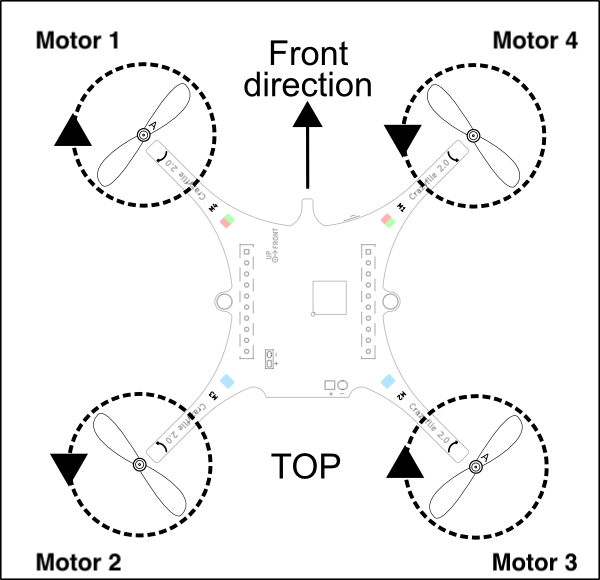
\includegraphics[height=3cm]{cf2_props}
        %\caption{Motors' controls}
        %\label{fig:crazyflie-motors}
    %\end{subfigure}
    %\hfill
    %\begin{subfigure}[t]{.49\linewidth}
     %   \centering
        %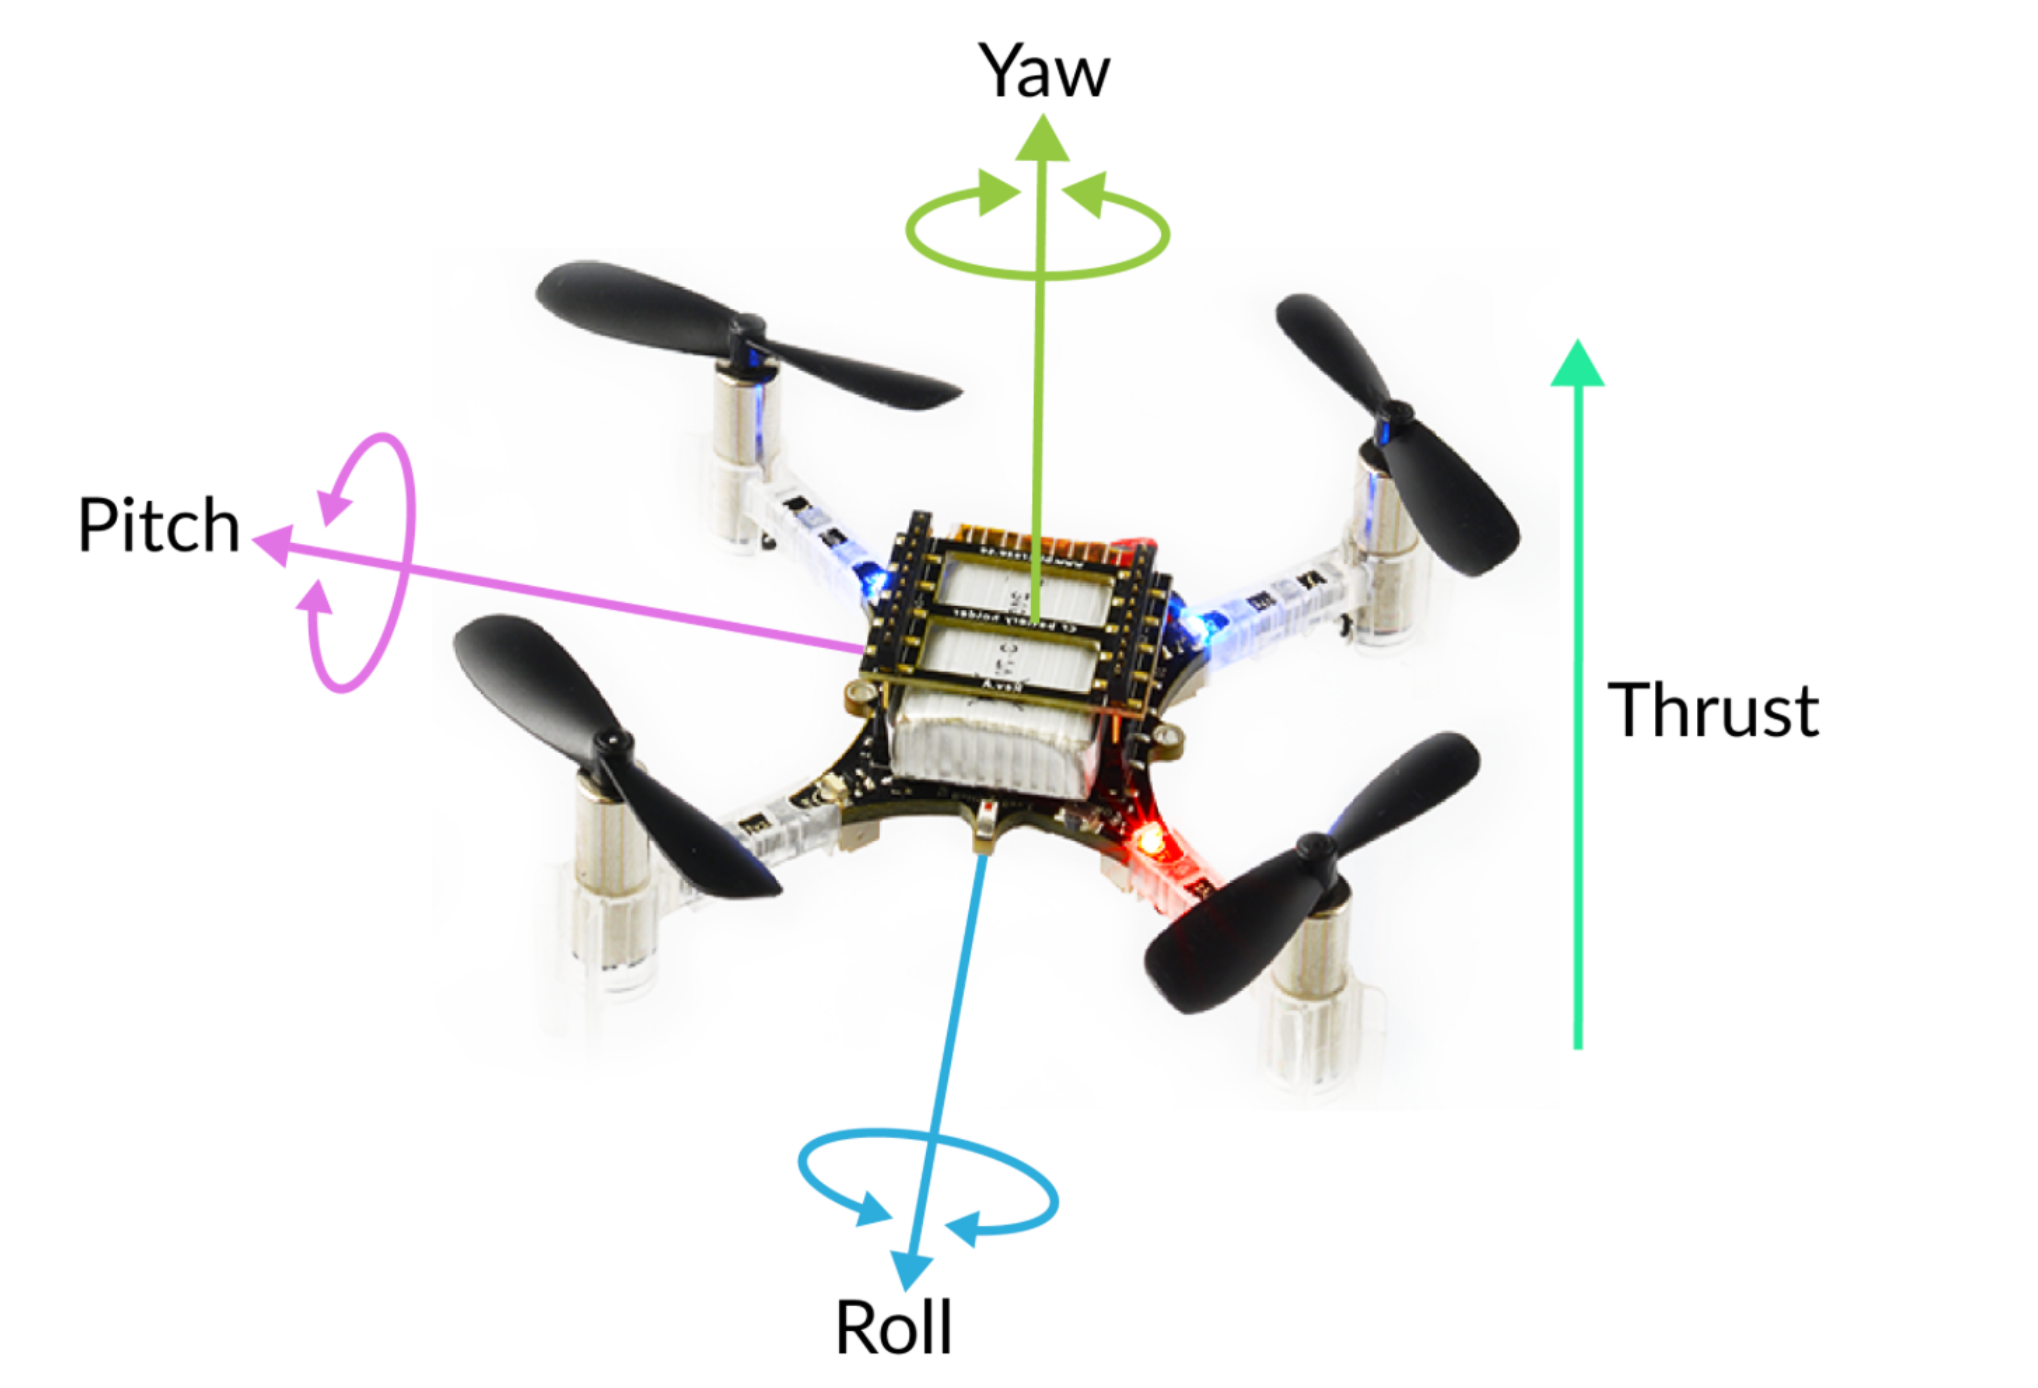
\includegraphics[height=3cm]{crazyflie2-axes}
        %\caption{Principal axes}
        %\label{fig:crazyflie-axes}
    %\end{subfigure}
    %\caption{Crazyflie 2.0 (excerpt from \cite{bitcraze})}
        %\label{fig:crazyflie}
%\end{figure}
%\todo{Figure from bitcraze, we might not be able to use this?}

We study the dynamics on the vertical axis and the pitch rate, roll rate and yaw rate control (4 degrees of freedom), with the following state variables: 
the vertical position in the world frame $z$,
the linear velocity of the center of gravity  
in the body-fixed frame with respect 
to the inertial frame $(u, v, w)$,
the angular orientation represented by the Euler angles $(\phi, \theta, \psi)$ where $\phi$ is the roll angle 
$\theta$ is the pitch angle and $\psi$ is the yaw angle, %(see \Cref{fig:crazyflie}),
the attitude or angular velocity with respect to the body frame $(p, q, r)$ with $p$ the roll rate, $q$ the pitch rate and $r$ the yaw rate.

%The Crazyflie 2.0 linear velocities are controlled through the angular velocities and the angular velocities are controlled through rotor thrust differential. For instance, to increase the pitch rate $q$, $Motor_2$ and $Motor_3$ rotor speeds should be higher than $Motor_1$ and $Motor_4$. As there is symmetry, it works similarly for the roll rate $p$ (with $Motor_4$ and $Motors_3$ vs. $Motor_1$ and $Motor_2$ instead). However, the yaw rate $r$ is controlled through the gyroscopic effect. To make the quadcopter rotate clockwise in the x-y plane, the rotor speeds of the clockwise rotating motors ($Motor_2$ and $Motor_4$) should be higher than those of the counterclockwise rotating ones ($Motor_1$ and $Motor_3$). \\
Using Newton's equations given a \emph{thrust} force and moments $M_x$, $M_y$ and $M_z$ exerted along the three axes of the quadcopter, 
and using the rotation matrix $R$ from the body frame to the inertial frame, 
%\begin{equation*}
%R = 
%\begin{pmatrix}
%c_\psi c_\theta & c_\psi s_\theta s_\phi -c_\phi s_\psi & s_\psi s_\phi +c_\psi c_\phi s_\theta \\
%c_\theta s_\psi & c_\psi c_\phi +s_\psi s_\theta s_\phi & c_\phi s_\psi s_\theta -c_\psi s_\phi \\
%-s_\theta & c_\theta s_\phi & c_\theta c_\phi
%\end{pmatrix}
%\end{equation*}
%\noindent (and $R^{-1}$ is the transpose of $R$) 
the Translation-Rotation kinematics and dynamics \cite{quadcopter_model} lead to a 10-dimensional non-linear dynamical system: 
%\todo{If we need space, could probably be formatted as two columns of 5 equations}
\begin{equation}
\label{eq:dynamic}
\left\{
\begin{alignedat}{2}
%\dot{x} &=(s_\phi s_\psi+c_\phi c_\psi s_\theta)w-(c_\phi s_\psi-c_\psi s_\phi s_\theta)v+c_\psi c_\theta u \\
%\dot{y} &=(c_\phi c_\psi+s_\phi s_\psi s_\theta)v -(c_\psi s_\phi-c_\phi s_\psi s_\theta)w+c_\theta s_\psi u \\
\dot{z} &= -s_\theta u + c_\theta s_\phi v + c_\theta c_\phi w &\qquad \dot{\theta} &= c_\phi q  - s_\phi r \\
\dot{u} &= rv - qw + s_\theta g & \dot{\psi}   &= \tfrac{c_\phi}{c_\theta} r + \tfrac{s_\phi}{c_\theta} q \\
\dot{v} &= -ru + pw - c_\theta s_\phi g & \dot{p} &= \tfrac{I_y - I_z}{I_x} qr + \tfrac{1}{I_x} M_x \\
\dot{w} &= qu - pv - c_\theta c_\phi g + \tfrac{F}{m} & \dot{q} &= \tfrac{I_z - I_x}{I_y} pr + \tfrac{1}{I_y} M_y \\
\dot{\phi}   &= p + c_\phi t_\theta r  + t_\theta s_\phi q & \dot{r} &= \tfrac{I_x - I_y}{I_z} pq + \tfrac{1}{I_z} M_z \\
\end{alignedat}
%\end{aligned}
\right.
\end{equation} 
\noindent
writing $c_{x}$ as a short for $cos(x)$, $s_{x}$ for $sin(x)$ and $t_{x}$ for $tan(x)$. 
$F$ is the sum of the individual motor thrusts, $I_x$, $I_y$, $I_z$ are the quadcopter's moments of inertial around the $x$, $y$ and $z$ axes, respectively. 

Instead of controlling directly each rotor speed, the four commands $thrust$, $cmd_{\phi}$, $cmd_{\psi}$ and $cmd_{\theta}$ are used to deduce the PWM values to apply to each motor, \Cref{eq:PWM}: 

\begin{equation}
\label{eq:PWM}
PWM = 
\begin{bmatrix}
  {PWM}_1 \\
  {PWM}_2 \\
  {PWM}_3 \\
  {PWM}_4
\end{bmatrix} = 
\begin{bmatrix}
  1 & -\nicefrac{1}{2} & -\nicefrac{1}{2} & -1\\
  1 & -\nicefrac{1}{2} & \phantom{-}\nicefrac{1}{2} & \phantom{-}1\\
  1 & \phantom{-}\nicefrac{1}{2} & \phantom{-}\nicefrac{1}{2} & -1\\
  1 & \phantom{-}\nicefrac{1}{2} & -\nicefrac{1}{2} & \phantom{-}1\\
\end{bmatrix}
\begin{bmatrix}
thrust \\
cmd_\phi \\
cmd_\theta \\
cmd_\psi \\
\end{bmatrix}
\end{equation} \\

PWMs are linked to rotation rates $\Omega$: 
%\begin{equation} 
%\label{eq:motor}
$   \Omega = 
%    \begin{bmatrix}
    [\omega_1 \ %&
    \omega_2 \ %&
    \omega_3 \ %&
    \omega_4 
%    \end{bmatrix}
]^\top
 = C_1 PWM + C_2$. 
%\end{equation}  
%\begin{equation} 
%   \Omega \odot \Omega =
%   \begin{bmatrix}
%    \omega_1^2 \\
%    \omega_2^2 \\
%    \omega_3^2\\
%    \omega_4^2 \\
%    \end{bmatrix} 
% = C_1^2(PWM \odot PWM) + 2C_1C_2PWM + C_2^2
%\end{equation}
Finally, we deduce the input force and moments from the squared rotation rates,  \Cref{eq:dynamic}, with force and momentum equations $[F \ M_x \ M_y \ M_z]^\top$ equal to:

\begin{equation} \label{eq:fulldynamic}
%\begin{split}
%\begin{bmatrix}
%F \\ M_x \\ M_y \\ M_z
%\end{bmatrix} 
%=
%  \begin{bmatrix}
%  C_T & C_T & C_T & C_T \\
%  -dC_T/\sqrt{2} & -dC_T/\sqrt{2} &dC_T/\sqrt{2} & dC_T/\sqrt{2}\\
%  -dC_T/\sqrt{2} & dC_T/\sqrt{2} &dC_T/\sqrt{2} & -dC_T/\sqrt{2}\\
%  -C_D & C_D & -C_D & C_D \\
%  \end{bmatrix}
%(\Omega \odot \Omega) \\
%=
\begin{bmatrix}
  C_T \big(C_1^2(cmd_{\theta}^2 + cmd_{\phi}^2 + 4cmd_{\psi}^2 + 4thrust^2) + 8C_1 C_2 thrust + 4C_2^2 \big)\\
  4C_Td\big(C_1^2 (cmd_{\phi}thrust - cmd_{\theta}cmd_{\psi}) +  C_1C_2cmd_{\phi} \big)  \\
  4C_Td\big(C_1^2 (cmd_{\theta}thrust - cmd_{\phi}cmd_{\psi}) +  C_1C_2cmd_{\theta}  \big)  \\
  2C_D\big(C_1^2(4cmd_{\psi}thrust - cmd_{\phi}cmd_{\theta}) + 4C_1C_2cmd_{\psi} \big)\\
\end{bmatrix} \\
%\end{split}
\end{equation}
\noindent The parameters are given in \Cref{sec:parameters}. 

 Given a series of controls (at time steps multiple of $dt\_commands$, 0.03 seconds here), the ODE of \Cref{eq:dynamic} %in \Cref{ode} 
can now be solved numerically (using Runge-Kutta of order 4 here, with a time step of 0.01 seconds) to obtain full quadcopter trajectories with high precision.


%This representation of commands is more closely related to attitude control than raw rotor speeds (or PWMs). $cmd_{\phi}$, $cmd_{\psi}$ and $cmd_{\theta}$ only control the roll rate $p$, the pitch rate $q$ and the yaw rate $r$, respectively. This direct mapping of commands to axes is more convenient to use for any type of controller.

\subsection{Motor failure}

\label{sec:motorfailure}

We suppose, for the sake of simplicity, that the quadcopter may experience a power loss on motor 1. 
This partial failure is modeled as a saturation of the maximum PWM, with a factor between 0.8 and 1.
%Always (nominal and non-nominal) saturation of the PID at 0.8 (to give slack to attitude control). 
%Only train in the small angle scenario. 

%We try with same saturation of the opposite motor (motor 4) and without. 

%Robustness of nominal, plus performance of the nominal/non-nominal training. 
 
Since quadcopter controls rely on differential thrust between motors, motor failures are very difficult to cope with. In order to keep a constant yaw when one motor is failing, the gyroscopic effect must be made equal to zero, for instance by having the two motors rotating in the opposite direction match the saturation of the faulty motor. The same idea applies to pitch and roll axes. 

Therefore, if the failure is not too harsh, and the target states are not too demanding, it is {\it a priori} feasible to recover some control of the faulty quadrotor by saturating all four motors in the same way. 

In this paper, we will look at two potential solutions to control in the presence of partial motor failure. The first one is to look at how robust a controller that has been designed for nominal cases (i.e. without partial motor failures) is. The other one is to train, using reinforcement learning, a controller optimized for a variety of situations, from no failure to maximal failure rate. 

%\todo{ What are the solutions ? Are they learned by the RL algo or are they based on principles like the one described here ? Wouldn't it be more accurate to say that we learn a controller under motor failure scenarios and try to see how different is the control algo from the one presented here?}

%In conclusion, the simplest solution is to apply the saturation to all four motors. However, to hover steadily, the Crazyflie 2.0 needs its four motors functioning at least at about 60\% of their maximum power. That is why $\alpha_{min} = 0.7$, so that the quadcopter keeps at least enough maneuverability to hover steadily. 

%More serious failures are considered in the literature, we refer the reader to \cite{failure,safe2ditch} for more detailed  measures (including 
%emergency landing procedures) that should be taken in these cases, and are orthogonal to our study here. 

%\todo{To be checked - safe2ditch - mention MRAC etc.? And the hopes that neural nets control can cope with that sort of things}

\subsection{Wind gusts}

\subsubsection{Aerodynamic effects}
\label{sec:aero}

In \Cref{eq:dynamic}, we neglected all aerodynamic effects. % to only keep as forces exerted on the quadcopter, gravity ($g$) and thrust ($F$), as well as Coriolis force due to the non Galilean referential (body frame). Similarly, torque was only produced by the angular velocities of the rotors $\Omega$, \Cref{eq:fulldynamic,eq:dynamic}.
When we take into account aerodynamic forces, an extra force $F^a$ is exerted on the quadcopter that depends on the wind speed and direction relative to the quadcopter, the angular velocities of the rotors and extra moments $M^a_x$, $M^a_y$ and $M^a_z$. We follow the full aerodynamic model of \cite{nanoquadcop} with the coefficients measured for a crazyflie 2.0, where the effect of the wind on the structure is neglected with respect to the effect on the rotors, and the blade flipping effect (due to elasticity of the rotor) is also neglected. %\todo{What's the rotor effect flipping?}

The extra force $F^a$ can be decomposed as the sum of the four extra aerodynamic forces on rotor $i$ ($i=1,\ldots,4$), that can be modelled as depending linearly on the rotors angular velocities, and linearly on the wind relative speed with respect to rotors. Other models \cite{Bangura} include blade flipping and other drag effects, but the induced drag we are modelling is the most important one for small quadrotors with rigid blades. % (and can even be simplified so that it does not depend on the angular speeds of rotors, see e.g. \cite{Bangura} again). 
We use $f^i= \Omega_i K W^r_i$  for the aerodynamic force exerted on rotor $i$ 
%\begin{equation*}
%  f^i = \Omega_i K W^r_i
%\end{equation*}
%\noindent 
in the inertial frame, where $K$ is the drag coefficients matrix, %, see \Cref{sec:parameters}, 
$W^r_i$ is the relative wind speed as seen from rotor $i$, in the body frame, i.e. $W^r_i=(u_i, v_i, w_i)-R^T W_a$ with $W_a$ the absolute wind speed in the inertial frame, $(u_i, v_i, w_i)$ being the linear velocities of the rotors in the body frame, $R$ is the rotation matrix from the body frame to the inertial frame ($R^T$ is its inverse, i.e. its transpose here), and $\Omega_i $ is the absolute value of the  angular velocity of the $i$-th rotor. 

On the crazyflie, $\Omega_i=C_1 PWM_i+C_2$, where $PWM_i$ are given using $thrust$, $cmd_{\phi}$, $cmd_{\theta}$ and $cmd_{\psi}$ using \Cref{eq:PWM}.

The linear velocities of rotors can be computed as follows:
\begin{equation*}
\begin{aligned}
\pmat{u_j \\ v_j \\ w_j} &= \pmat{p \\ q \\ r}
  \times \pmat{d c_j \\ d s_j \\ h} + \pmat{u \\ v \\ w} 
  &=
  \begin{pmatrix}
    \phantom{-}qh-rds_j+u \\
    -ph+rdc_j+v \\
    pds_j-qdc_j+w
  \end{pmatrix}
\end{aligned}
\end{equation*}
\noindent where $(u,v,w)$ are the linear velocities of the
center of mass of the quadrotor in the body frame, $(p,q,r)$ are the angular velocities of the quadrotor, $d$ is the length of the arm linking the center of the drone to any of the four motors, and for $j \in \{1, 2, 3, 4\}$, 
$c_j=sin\big(\frac{\pi}{2}(j-1)+\frac{3\pi}{4}\big)$ and $s_j=cos\big(\frac{\pi}{2}(j-1)+\frac{3\pi}{4}\big)$ are such that  $(c_j,s_j,h)$ is the coordinate of rotor $j$ in the body frame, with the center of mass being the origin.

Now, we add to the second term of \Cref{eq:dynamic} for $\dot{u}$, $\dot{v}$, $\dot{w}$ the aerodynamic force $F^a=(F^a_x,F^a_y,F^a_z)$ divided by $m$, and to moments of \Cref{eq:fulldynamic}, the aerodynamic moments $M^a=(M^a_x, M^a_y,$ $M^a_z)$ with 
$F^a  = f_1+f_2+f_3+f_4$
and $M^a = (dc_1,ds_1,h)\wedge f_1 + (dc_2,ds_2,h) \wedge f_2
      + (dc_3,ds_3,h)\wedge f_3+(dc_4,ds_4,h) \wedge f_4$.

%\begin{equation*}
%\begin{aligned}
%F^a & = f_1+f_2+f_3+f_4\\
%M^a & = (dc_1,ds_1,h)\wedge f_1 + (dc_2,ds_2,h) %\wedge f_2\\
%    & \qquad + (dc_3,ds_3,h)\wedge f_3+(dc_4,ds_4,h) \wedge f_4
%\end{aligned}
%\end{equation*}
%-F^a_1-F^a_2+F^a_3+F^a_4 \\
%M^a_y & = & -F^a_1+F^a_2+F^a_3-F^a_4 \\
%M^a_z & = & -F^a_1+F^a_2-F^a_3+F^a_4 \\
%\todo{Pb on $z$ component, see equation for $M_z$}
%This, together with \Cref{eq:dynamic} gives 
We derive the full dynamics of the quadcopter considering aerodynamic effects, and only write below the modified equations: 
\begin{equation}
\label{eq:aerodynamic}
\left\{
\begin{alignedat}{2}
%\dot{x}=(s_\phi s_\psi+c_\phi c_\psi s_\theta)w-(c_\phi s_\psi-c_\psi s_\phi s_\theta)v+c_\psi c_\theta u \\
%\dot{y}=(c_\phi c_\psi+s_\phi s_\psi s_\theta)v -(c_\psi s_\phi-c_\phi s_\psi s_\theta)w+c_\theta s_\psi u \\
%\dot{z} = -s_\theta u + c_\theta s_\phi v + c_\theta c_\phi w \\
\dot{u} &= rv - qw + s_\theta g + \tfrac{F^a_x}{m} & \dot{p} &= \tfrac{I_y - I_z}{I_x} qr + \tfrac{1}{I_x} (M_x+M^a_x) \\
\dot{v} &= -ru + pw - c_\theta s_\phi g\!+\!\tfrac{F^a_y}{m} &\quad \dot{q} &= \tfrac{I_z - I_x}{I_y} pr + \tfrac{1}{I_y} (M_y+M^a_y) \\
\dot{w} &= qu - pv - c_\theta c_\phi g\!+\!\tfrac{F+F^a_z}{m} &  \dot{r} &= \tfrac{I_x - I_y}{I_z} pq + \tfrac{1}{I_z} (M_z+M^a_z) \\
%\dot{\phi} = p + c_\phi t_\theta r  + t_\theta s_\phi q \\
%\dot{\theta} = c_\phi q  - s_\phi r \\
%\dot{\psi} = \frac{c_\phi}{c_\theta} r + \frac{s_\phi}{c_\theta} q \\
\end{alignedat}
\right.
\end{equation} 

\subsubsection{Wind models}

There are two main types of models in the litterature, represented by e.g. Discrete Wind Gust and von K\'arm\'an Gust or Dryden Gust models. Von K\'arm\'an gusts and Dryden gusts are stochastic gust models (homogeneous and stationary gaussian processes) characterized by their power spectral densities for the wind's three components, Dryden gusts being an approximation of Von K\'arm\'an gusts. 

The Discrete Wind Gusts model consists in a explicit and deterministic representation of wind gusts as half period cosine perturbations (\cite{demourant1}, eq. (45)) detailed below.
%in \Cref{gust}. 
We focus on this model because it is widely used for aircraft certification (using dozens of discrete wind gusts with different magnitudes and scales). 

A discrete wind gust is characterized by its fixed direction, magnitude and scale, and lasts for a half period during which wind speed increases until it reaches its maximum intensity. The absolute wind velocity is given as a function of time as, using the same notations as in \Cref{sec:aero}:
%\begin{equation}
%\label{gust}
$W_a(t) =
%\begin{cases}
%  0 & t < t_0\\
  \frac{A_g}{2} \left(1 - cos\big(\frac{\pi (t-t_0)}{\delta}\big)\right) V_d$ if $  t_0 \leq t \leq t_0+2\delta$, 0 otherwise, 
%  0 & t > t_0+2\delta
%\end{cases}
%\end{equation}
where $A_g$ is the maximal magnitude of the wind gust, $\delta$ is the half life of the gust, and $V_d$ is a normalized vector in $R^3$, which is the wind (absolute) direction. 
        
%Proposition : $A_g\leq 3 m.s^{-1}$, $\delta\leq 0.5s$, $V_{d}$ normalized vector in $R^3$. 
 
\subsection{PID Control}

As in \cite{rl}, the objective is to train only the attitude controller, and not the altitude one. We therefore use a PID for controlling $z$. We will also need some idea of what a standard PID controller may achieve in terms of performance, and robustness to wind gusts and failures. For this, we will primarily use one of the altitude and attitude PID controller implemented in the crazyflie 2.0. 
Given setpoints $z_{sp}$, $p_{sp}$, $q_{sp}$ and $r_{sp}$, the quadrotor is controlled using a PID controller (called PID1 in the sequel) which is the one of \cite{goubault_putot} (see Appendix \ref{sec:parameters}). 
%given by \Cref{eq:control1}, see e.g. %\cite{goubault_putot}, that we call PID1:
%\begin{equation}
%\label{eq:control1}
%\left\{
%\begin{aligned}
%thrust &= 1000 \big(25(2(z_{sp} - z) - w) \\ & \qquad + 15 \smallint (2(z_{sp} - z) %- w)\dt\big) + 36000 \\
%cmd_{\phi} &= 250 (p_{sp} - p) +  500 %\smallint (p_{sp} - p) \dt \\
%cmd_{\theta} &= 250 (q_{sp} - q) +  500 %\smallint (q_{sp} - q) \dt \\
%cmd_{\psi} &= 120 (r_{sp} - r) + 16.7 %\smallint (r_{sp} - r) \dt
%\end{aligned}
%\right.
%\end{equation}

But as we will see, the attitude controller implemented in the crazyflie 2.0 is not very reactive, most probably for ensuring that the altitude is very securely controllable (since too much reactivity in pitch and roll means sudden loss of vertical speed). In order to give an idea of what we could observe as best performance, we 
also designed a specific PID for attitude, that we call PID2, which is much more reactive:  %shows much more aggressiveness:


\begin{equation}
\label{eq:control2}
\left\{
\begin{aligned}
thrust &= 3000(z_{sp} - z) \\ & \qquad + 300 \smallint (z_{sp} - z) \dt - 500 \dot{z} + 48500 \\
cmd_{\phi} &= 1000 (p_{sp} - p) +  400 \smallint (p_{sp} - p) \dt - 40 \dot{p} \\
cmd_{\theta} &= 1000 (q_{sp} - q) +  400 \smallint (q_{sp} - q) \dt - 40 \dot{q}\\
cmd_{\psi} &= 2000 (r_{sp} - r) + 1000 \smallint (r_{sp} - r) \dt - 100 \dot{r}
\end{aligned}
\right.
\end{equation}

\section{Training}

\label{sec:training}

\subsection{Underlying Markov decision process}

\label{sec:Markov}

Reinforcement learning is designed to solve Markov decision problems. At each discrete time step $k=1, 2, \ldots$, the controller observes the state $x_k$ of the Markov process, selects action $a_k$, receives a reward $r_k$, and observes
the next state $x_{k+1}$. As we are dealing with Markov processes, the probability distributions for $r_k$ and $x_{k+1}$ depend only on $x_k$ and $a_k$. Reinforcement learning tries to find a control policy, i.e. a mapping from states to actions, in the form of a neural net, that maximizes at each time step the expected discounted sum of future reward. 

For the attitude control problem at hand, the set of Markovian states is $thrust$, $p$, $q$, $r$, $err_p=p_{sp}-p$, $err_q=q_{sp}-q$, $err_r=r_{sp}-r$ (where $(p_{sp}, q_{sp}, r_{sp})$ is the target state, or "plateau" we want to reach), in the nominal case (similarly to what is done in e.g. \cite{Koning}). We will also consider partially observed Markov processes, with only subsets of states for improving sampling over smaller dimensional states, by leaving out those states which should have less influence on the dynamics: our first candidate is to leave out thrust, which appears only as second order terms in the moments calculation, \Cref{eq:fulldynamic}, and also, $p$, $q$, $r$ that are second order in the formulation of the angular rates, again in \Cref{eq:fulldynamic}. %In the hope for getting smoother decisions, we also test a 13-dimensional \todo{Maybe maybe not?} state in Section \ref{sec:experiments}, comprising the Markovian states but also the linear velocities $u$, $v$, $w$ and past commands $cmd_\phi$, $cmd_\theta$ and $cmd_\psi$. 
We do not consider here adding past information, classical in non Markovian environments \cite{NMR}, that has been used for attitude control in e.g. \cite{rl}, but increases the dimension by a large amount. 

%In non-nominal cases, we have to add some amount of information to the observed states. 
In the case of partial motor failure, we add the knowledge of the maximum thrust for faulty motor 1, as a continuous variable between 80\% and 100\%. In the case of aerodynamic effect and wind gusts, we add the knowledge of the maximal magnitude and direction (in the inertial frame) of the incoming wind. In both cases, it can effectively be argued that it is possible to detect failures in almost real time, and to measure (or be given from ground stations) maximum winds and corresponding directions, in almost real time as well. In the case of wind-gusts, Markovian states include also the linear velocities $u$, $v$ and $w$, since wind gusts are only defined in the inertial frame, and the induced aerodynamic effects depend on relative wind speed. 

With a view to solving optimal control problems (or Model-Predictive like control), we choose to use a reward function 
%(the opposite of the cost to be minimized in optimal control) 
which is a measure of the distance between the current attitude $(p,q,r)$ with the target attitude $(p_{sp}, q_{sp}, r_{sp})$ (similar to the one used in \cite{rl}): 
$r(s) = - max\left(0, min\left(1, \frac{1}{3\Omega_{max}} \left\lVert \Omega^* - \Omega \right\rVert\right)\right) $, 
\noindent $\Omega_{max}$ being the maximal angular rate that we want to reach for the quadcopter, and $\Omega$ is the angular rate vector $(p,q,r)$ which is part of the full state $s$ of the quadcopter.

%\todo{Do we want to test same reward + smoothing term ($-\alpha | | cmd | |_2$ normalized by $\alpha$ so that this does not go beyond $1/2$; so $\alpha=(400^2+400^2+1000^2)/2$)?}

\subsection{Neural net architecture}

\label{sec:neuralnetarchi}

Neural nets, such as multiple layer perceptrons (MLP) with RELU activation, can efficiently encode all piecewise-affine functions \cite{RELUnet}. It is also known \cite{MPC} that the solution to a quadratic optimal control (MPC) problem for linear-time invariant system is piecewise-affine. Furthermore, there are good indications that this applies more generally, in particular for non-linear systems \cite{nonlinearmpc}. This naturally leads to thinking that MLPs with RELU networks are the prime candidates for controlling the attitude with distance to the objective as cost (or reward). In some ways, the resulting piecewise-affine function encodes various proportional gains that should be best adapted to different subdomains of states, so as to reach an optimal cumulated (and discounted, here with discount rate $\gamma=0.99$) distance to the target angular rates, until the end of training.
%(1 second as we will see in \Cref{subsec:training}). 
%\todo{Difficult to explain the last tanh layer in that presentation...I will try}

In theory \cite{Ferlez}, one could find a good indication of the architecture of the neural net in such situations, but the bounds  that are derived in \cite{Ferlez} are not convenient for such a highly complex system. It is by no means obvious what architecture will behave best, both for training and for actual controller performance, although a few authors argue that deeper networks should be better, see e.g. 
\cite{LUCIA2018511}. 

Architectures that have been reported in the literature for similar problems are generally alike. 
In \cite{simtoreal}, 
the neural net is a Multi-Layer Perceptron (MLP) with two layers of 64 neurons each, and with $\mathrm{tanh}$ activation function. % trained using Proximal Policy Optimization \cite{PPO}.
In \cite{fei2020learn}, the part of  the controller which is a neural net is a MLP with two layers of 96 neurons each and $\mathrm{tanh}$ activation function, % trained using Deep Deterministic Gradient Policy, 
whose input states (observation space) are all states plus the control. 
In \cite{Koning}, the hover mode neural net controller, which is the most comparable to our work, is a MLP with two layers of 400 and 300 neurons respectively, with RELU activation for hidden layers and $\mathrm{tanh}$ for the last layer. 
In \cite{stockholm}, the resulting architecture is a two layers MLP with 128 neurons on each layer, and RELU activation function. 

%\todo{Reporter une partie sur les sections suivantes}

%HUP

We will report experiments with one to four layers, and with 4, 8, 16, 32 or 64 neurons per layer, with RELU activation function (except for the rescaling of the output, using $\mathrm{tanh}$). We limit the reporting of our experiments to these values since we observed that these were enough to find best (and worst) behaviours. 

\subsection{Training algorithms}

\label{subsec:training}

The first three algorithms we are discussing in \Cref{sec:experiments}, DDPG \cite{DDPG}, SAC \cite{SAC} and TD3 \cite{TD3} are all off-policy, actor-critic methods, which are generally considered to be better suited for control applications in robotics \cite{Sutton} (DDPG is used for instance in \cite{fei2020learn}). Because of its effectiveness in practice, observed by many authors, e.g. \cite{rl} for attitude control, we also compare with the on-policy 
Proximal Policy Optimisation \cite{PPO}, also used  for similar applications in 
\cite{simtoreal} and  
in \cite{stockholm}. 

%Position control (x, y, z) for the crazyflie? ; seems to be only Roll+pitch and yaw rate+wanted thrust? control (chapter 5, small angles). Motor and mass are within intervals (weight load, degraded motors). Extension of PPO (robust PPO) ; discount factor of 0.95 see other parameters in Table 5.1. L1 and entropy regularization are used. [128,128] RELU. 
% HUP

DDPG is the historical method for continuous observation and action space applications to control, SAC and TD3 being later improvements of DDPG. For instance, 
SAC regularizes the reward with an entropy term that is supposed to reduce the need to fine hyper-parameter tuning. 

%\todo{The relation between the sentence below and the definition of the classes of query is unclear}
\todo{Also, should not this be part of the experimental setup? EG: would be better, but difficult since we want to mention also that this has been considered for training, so for now I leave this as is}
Let us now describe the training mechanism: we call {\it query signal} the function describing the prescribed angular rates at any given time. %\todo{please check I correctly explained} 
We model this signal by a constant plateau, of magnitude chosen randomly between -0.6 and 0.6 radians per second, and duration chosen randomly between 0.1 and 1 second. We are training over a time window of 1 second (a training episode) during which the query signal is a constant plateau followed by a value of 0 until the end of the episode.
We chose to report on training where these query signals are used independently on pitch, roll and yaw. Having joint queries on pitch, roll and yaw does not seem to change the outcome of our experiments. 

Controls are updated every 0.03 seconds, and we simulate the full state of the quadrotor, using a Runge Kutta of order 4 on \Cref{eq:dynamic} with a time step of 0.01 seconds. 

%\todo{Something we could discuss, or try later (probably no time before the deadline), regularization, or changing the architecture of the neural net (not dense MLP, adding a CNN part with feature extraction etc.). }

%\todo{Explain episodic and continuous tasks}
The evaluation of the controller is made on similar query signals, but on time windows that last 20 seconds, with a query signal generated according to a more general class of queries (see below). 
Query signals on such longer time windows could also be considered for training : \cite{rl} refers to this approach as "continuous mode" and reports much poorer performance compared to the "episodic mode" with 1 second queries. We therefore decided to report only on episodic mode training. 
%We decided to only report here the training on one query of 1 second as described above ("episodic" mode in \cite{rl}) and not in the continuous mode (20 seconds, with many different target states) 
%as this continuous mode appears to have very bad performance, as already observed in \cite{rl}. 
%\todo{Changed the sentence completely, EG please check}
%\todo{I'm confused about this sentence: aren't we showing results on 20-sec episodes in the graphs? what we really mean is to explain why we train on shorter episodes rather than on the full 20-sec episodes, as used for evaluation? please confirm so I can improve the sentence ; EG: I have made the change - this is correct, is that more understandable?}

%\todo{Arthur?}

Such query classes are characterised by three distributions $A$, $D$ and $S$ for respectively the amplitude and duration of stable plateaus, and the step amplitude between successive stable plateaus. These distributions are the same for each axis.
We define three different classes of queries (where U(a,b) denotes the Uniform distribution of support [a,b]):
%\begin{itemize}
    %\item 
    easy (A = U(-0.2, 0.2), D = U(0.5, 0.8), S = U(0, 0.3)), 
    %\item 
    medium (A = U(-0.4, 0.4), D = U(0.2, 0.5), S = U(0, 0.6)) and 
    %\item 
    hard (A = U(-0.6, 0.6), D = U(0.1, 0.2), S = U(0, 0.9)). 
%\end{itemize}
Our query generator actually changes the joint distribution of amplitude and duration of stable plateaus by filtering out those queries which would make the roll, pitch and yaw go through singular values in the Euler angles description of the dynamics. 
%the acceptable states, see \Cref{params1}\todo{Check?}. 


%The intersection of the query classes is null.

\section{Formal performance criteria}
\label{sec:perf-observers}

Designing a controller for a specific application requires balancing multiple criteria such as rising time, overshoot, steady error, etc. 
In order to quantify rigorously the performance of the learned controller, we formalized requirements using a recent extension of 
Signal Temporal Logic (STL) published in \cite{2019bakhirkinbeyondstl}, interpreted over piecewise constant signals.
In addition to the usual \emph{Globally}, \emph{Finally} and \emph{Until} modalities, this logic offers:

\begin{itemize}
\item  $\On_{[a,b]} ~ \Agg  ~ \tau(x)$, with $\Agg \in \{\MinAgg, \MaxAgg\}$, which computes a Min/Max aggregate of a real-valued term $\tau(x)$ on time interval $[a,b]$;

\item $\tau(x) ~ U_{[a,b]}^d ~ P(x)$, which samples the term $\tau(x)$ when $P(x)$ first becomes true within $[a,b]$, or returns the default value $d$ if $P(x)$ does not become true in $[a,b]$;

\item $D_{a}^d \tau(x)$ which samples the value of term $\tau(x)$ (or formula $P(x)$) at time $a$ if it is defined, or returns $d$ otherwise;

\item $\ite(P(x), \tau_1(x), \tau_2(x))$ which is equal to $\tau_1(x)$ when $P(x)$ is true and to $\tau_2(x)$ otherwise.
\end{itemize}

A first set of formulae allows to identify instants when a query signal $q$ becomes stable for $T$ time units, 
and whether $q$ goes up or down at any instant (with $\epsilon$ and $d$ two small constants), and the step size:
\begin{align}
       \stable(q) &= (\On_{[0, T]} ~ \MaxAgg ~ q) - (\On_{[0, T]} ~ \MinAgg ~ q) < d\\
\becomesstable(q) &= (D_{-\epsilon}^\bot ~ \lnot \stable(q)) \land \stable(q)\\
           \up(q) &= q - (D_{-\epsilon}^0 ~ q) > 0 \\
         \down(q) &= q - (D_{-\epsilon}^0 ~ q) \leq 0 \\
        \stepSize(q) &= \ite(\becomesstable(q), q - D_{-\epsilon}^0{q}, 0) 
\end{align}

We consider an angular rate signal $x$ as acceptable if it does not overshoot a stable query $q$ 
by more than $\alpha\%$ of the step size on $[0, T_1]$, and does not stray away from a stable query $q$ 
by more than $\beta\%$ of the step size on $[T_1,T]$:
\begin{align}
\becomesstable(q) \land \up(q)   &\implies \On_{[0, T_1]} ~ \MaxAgg ~  (x - q)  < \alpha \stepSize(q) 
\label{eq:overshootup} \\
\becomesstable(q) \land \down(q) &\implies \On_{[0, T_1]} ~ \MaxAgg ~  (q - x)  < \alpha \stepSize(q) 
\label{eq:overshootdown}\\
\becomesstable(q)                &\implies \On_{[T_1, T]} ~ \MaxAgg ~ \|x - q\| < \beta \stepSize(q)
\label{eq:offset}
\end{align}

We define the rising time $\mathit{RT}$ as the time it takes for $x$ to first reach $q$ within $\gamma\%$:
\begin{equation}
\ite(\becomesstable(q),  t - (t ~ U_{[0,T]}^{+\infty} ~ \|(x-q)\| < \gamma q), +\infty)
\label{eq:rising}
\end{equation}

\Cref{fig:observer-params} illustrates the formalised notions and parameters.
\begin{figure}[htbp]
    \centering
    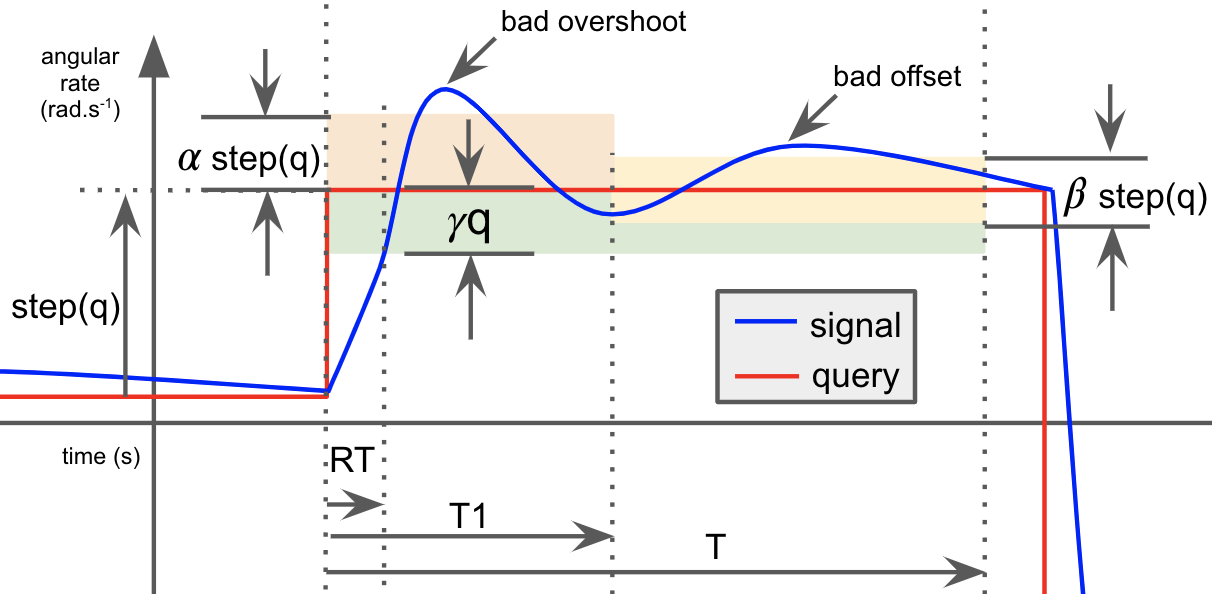
\includegraphics[width=\linewidth]{observer-params}
    \caption{Property parameters $T_1$, $T$, $RT$, $\alpha$, $\beta$, $\gamma$.}
    \label{fig:observer-params}
\end{figure}

Using observers code generated from these specifications, we compute statistics about property violations 
and associated robustness margins on angular rate signals and queries on pitch, yaw and roll axis of the system, 
acquired at regular intervals during the training of the controller. For evaluation each property $P(x,q)$ is wrapped 
in a \emph{globally} modality over the episode length yielding $G_{[0,\mathit{episode\_length}]} ~ P(x,q)$.
Automating the computation of these behavioral metrics is essential in allowing to scale up the hyper-parameter
space exploration and identify the best controller according to objective measurements. 

\section{Experimental setup}

\label{sec:experiments}

\subsection{Implementation}

We have developed a platform with the purpose of running experiments in a reproducible and scalable way, becoming an integration layer between the different moving parts in both training and testing.
From a technological standpoint the platform is based on the Stable Baselines 2.7.0 reinforcement learning library \cite{stable-baselines} itself based on Tensorflow \cite{abadi2016tensorflow}, all of our code is in Python and we used Bazel \cite{Bazel} as build system. We used Tensorboard to monitor losses and the internal dynamic of the neural networks during the training.
%\todo{NB: I think the following could be moved into the appendix as an implementation detail}

One intermediate goal was to explore the large combinatorial hyperparameter space efficiently to be able to identify the best hyperparameters values with respect to the STL metrics we defined and to get a better understanding of their impact.

With 4 different algorithms, 20 possible configurations for the network architecture and 3 sets of observed states, our hyperparameters space contains a total of 240 points that need to be trained and tested. The corresponding jobs are dispatched on our Kubernetes cluster \cite{Kubernetes} where they can run in parallel. Disposing of 1 vCPU on the Cascade Lake platform (base frequency of 2.8 GHz), the 3 millions iterations of a single training job take between 3 and 8 hours to complete. The cluster autoscales with the workload and allowed us to run 1200 hours worth of training in half a day.

The container images that end up running on the cluster are created, uploaded and finally dispatched in a reproducible manner thanks to the Bazel rules of our Research Platform. Those rules are built on top of the Bazel Image Container Rules \cite{bazel-rules-docker} and the Bazel Kubernetes Rules \cite{bazel-rules-k8s} and specially designed to generate all the experiment jobs of the hyperparameters analysis.

The training and testing results are automatically uploaded on our cloud storage where they can be browsed for quick inspections, or fed as input for the next pipeline stage.
We saved 30 checkpoints per experiment (each file containing 100k training iterations weights between 10KB and 100KB). Including the TensorFlow logs, the training results amount to >100GB of data.

%We organized these jobs in rounds and each round, consisting of approx N training jobs each corresponding to a specific point in the hyperparameters space.
%We trained each of these networks for 3M iterations and saved checkpoints every 100k iterations hence having 30 checkpoints per experiment, each checkpoint is between 10KB and 100KB.
%Training one round on a K8S cluster with this characteristics took about K hours and produced a total of 30xN checkpoints to be evaluated and D amount of gigabytes, also including the Tensorflow logs.
Each of the 30 $\times$ 240 checkpoints was then evaluated on 100 queries computed by the Query Generator, producing the same number of concrete traces representing the commands and the states over the whole episode. Each set of such traces is about 600k hence it yields total of 60MB per checkpoint. %and took K hours on the same kind of platform used for the training.
Finally each of the 30 $\times$ 240 $\times$ 100 traces was evaluated with STL properties observer to compute synthetic metrics: aggregating the 100 traces of a single checkpoint produced a 150KB file and required approximately 45 minutes.
The checkpoint specific CSV files were further aggregated in experiment specific and round specific checkpoints for the final visual inspection.


\subsection{Interactive browsing of the experiments database}

%\todo{Put ref to hiplot and one screenshot explained quickly}

We want to understand what correlations we have between controller performance and the way it has been trained, and for this, we used Hiplot
\cite{hiplot} for browsing through the enormous number of parameters and data generated. 
We show in \Cref{fig:hiplot} how we used Hiplot in an interactive manner for verifying our hypotheses. Each parameter and performance measure is represented by a column in the graph generated by Hiplot from our database. For each parameter, either fixed or free, choosing intervals of values for each performance measure creates lines that link parameter values to performance values within the chosen intervals. The number of entries in the database (i.e. the number of controllers) that satisfy the constraints is also shown, as well as the table of all their corresponding parameters and performance values. 

\begin{figure}
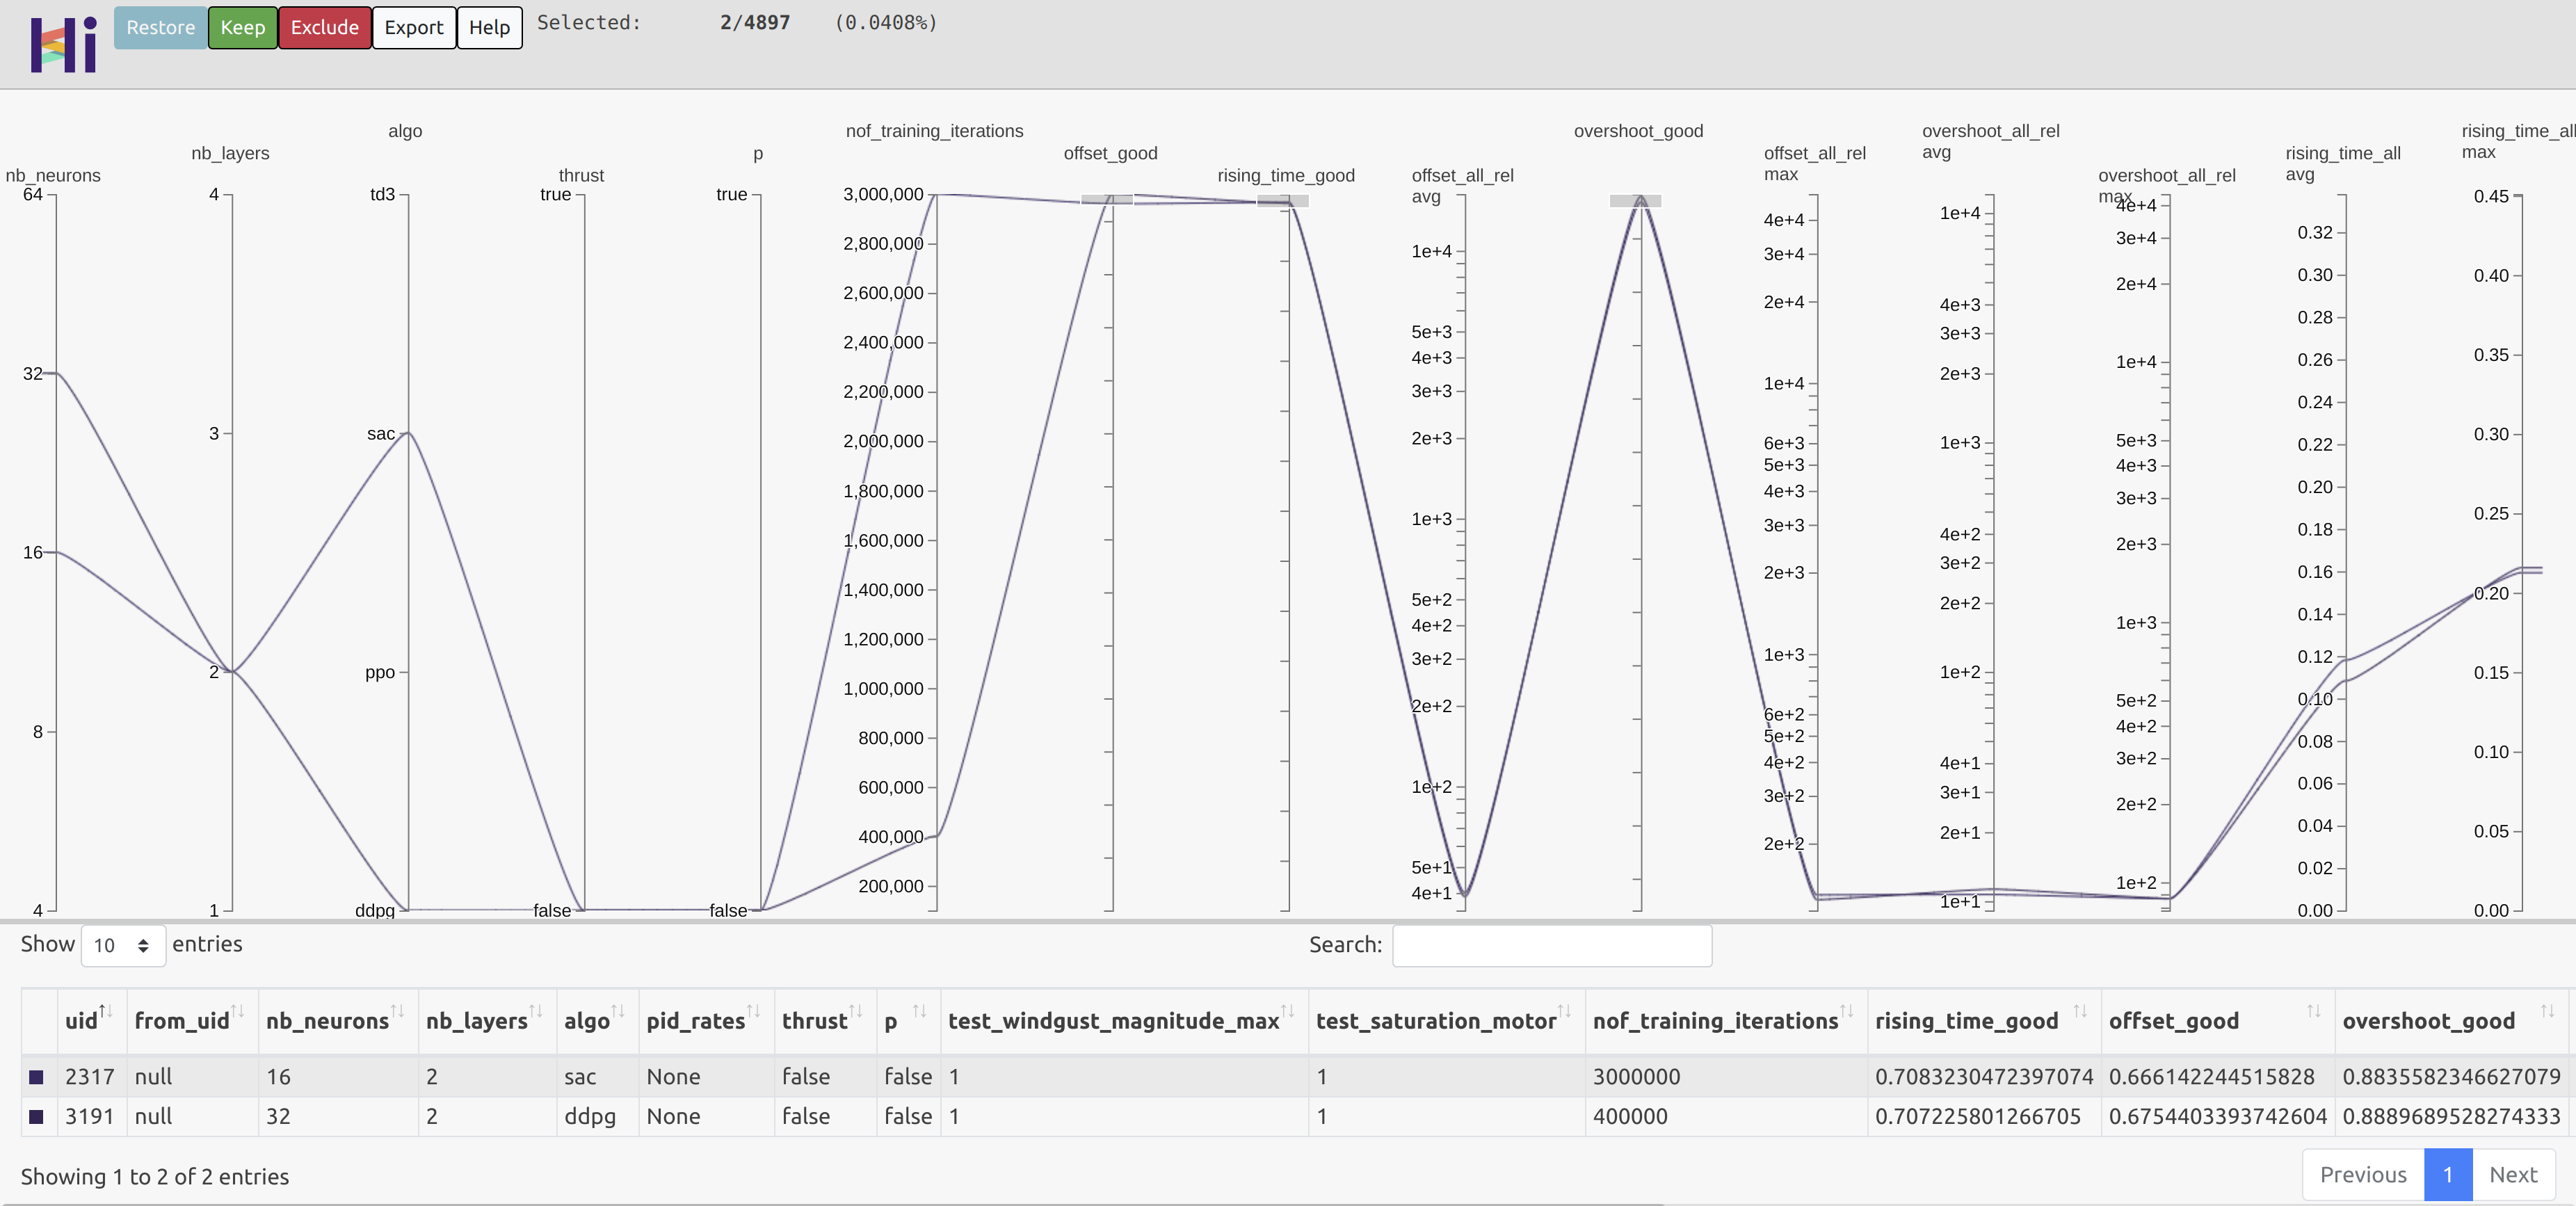
\includegraphics[width=\linewidth]{hiplot_better_networks}
\caption{Hiplot interactive session}%Sample neural net (1 layer of 8 neurons) command trajectory and its corresponding target angular rates trajectory.}
% Here SAC 32x32 3M iterations 3 states
\label{fig:hiplot}
\end{figure}
For instance, we used Hiplot to select the "best" networks,  filtering the data set of controllers, only retaining the ones with better success in offset, overshoot and rising times altogether, with respect to the best PIDs.
%on the three measures on overshoot, offset and rising time
%"OK overshoot", "OK off." and "OK rising t.". 
This resulted in two neural nets with much better performances than the PIDs on offset and on rising time as we will discuss in \Cref{sec:exp-results}.
%\todo{Which ones Arthur? SAC 16x16 how many iterations? DDPG 32x32 how many iterations?}
%\todo{future availability of implem?}

\section{Experiments results}
\label{sec:exp-results}
\subsection{Performance metrics}

Each controller is evaluated on a hundred evaluation episodes using STL observers defined in \Cref{eq:overshootup,eq:overshootdown,eq:offset,eq:rising},
where parameters are set to $\alpha=10\%$, $\beta=5\%$ and $\gamma=5\%$, $T=0.5s$, $T_1=0.25s$, $\epsilon = 0.01s$, $d=0.005$.
For each evaluation episode the following statistics are computed over all stable query plateaus: 
\begin{itemize}
\item average and maximum overshoot percentage relative to the query step size, 
\item average and maximum offset percentage relative to the query step size, 
\item average and maximum rising time values in seconds (only for plateaus where the signal actually reaches $\gamma\%$ of the query within $[0,T]$).
\end{itemize}

For each metric (overshoot, offset, rising time), we compute the \emph{success percentage} {\% OK}, i.e. the percentage of stable plateaus of the episode for which the controller behaviour satisfies the specification.

Then, episode-level statistics are further averaged, yielding results presented in the tables of the following sections, where columns represent:
\begin{itemize}
    \item avg (resp. max) overshoot: is the per-episode-average of the average (resp. maximum) overshoot values,
    \item avg (resp. max) offset: is the per-episode-average of the average (resp. maximum) offset values,
    \item avg (resp. max) rising time: is the per-episode-average of the average (resp. max) rising time, 
    \item \% Ok offset (resp. overshoot, rising time): is the per-episode-average of the success percentage for the offset (resp overshoot, rising time) metric. 
\end{itemize}


\subsection{Performance of nominal-trained networks in nominal test case}
\label{sec:expnominal}
%Start with PIDs performance description, extract thresholds for the neural controllers analysis.

%As usual with PIDs, rising time is best (lowest) corre     sponds to overshoot being worst (highest). 

%\begin{csvtable*}{PIDs_nominal.csv}
%\caption{Performance of the PIDs}
%\label{fig:pidnominal}
%\end{csvtable*}

%\subsubsection{Simple observations on neural net training}

\subsubsection{Overall best performance comparison}
The PID performance metrics in the nominal case are reported in the first two lines of \Cref{fig:pidnnnominal} to serve as a reference point for neural controller evaluation.
Examples of query tracking behavior are given in \Cref{fig:pid_traces} for reference.

\begin{figure}
%\begin{subfigure}{18cm}
%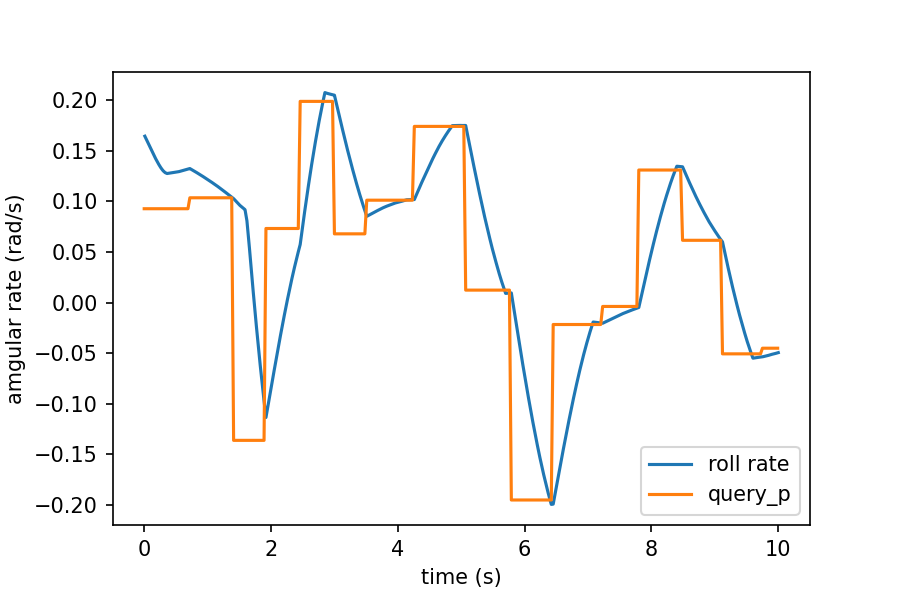
\epsfig{file=pid1.png,clip=,width=18cm}
%\caption{PID1 controller}
%\end{subfigure}
%\begin{subfigure}{18cm}
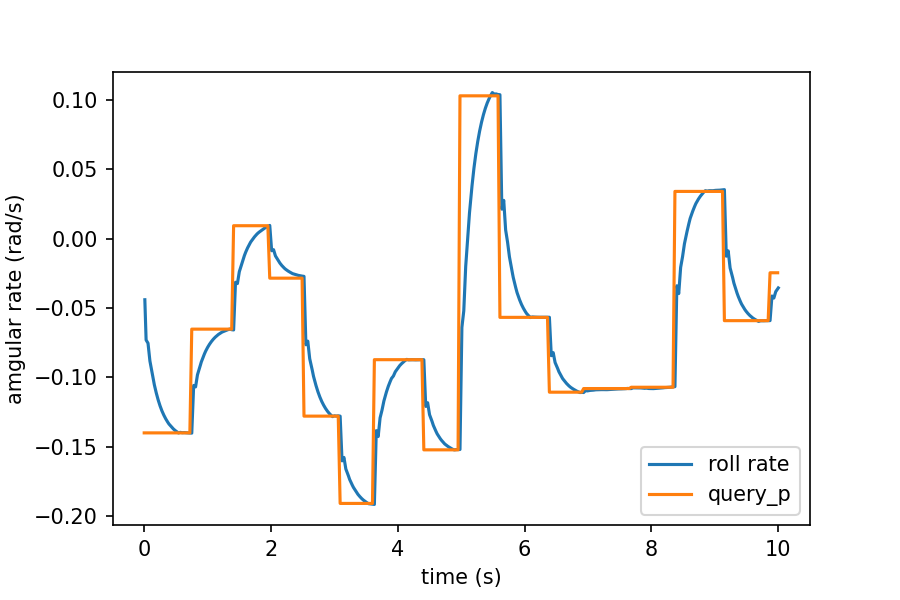
\epsfig{file=pid2.png,clip=,width=0.5\textwidth}
\caption{PID2 controller query tracking}
%\end{subfigure}
%\caption{Query tracking behaviour for PID controllers.}
\label{fig:pid_traces}
\end{figure}

PID2 reaches within 5\% of the target state for about 70\% of the queries, and is relatively slow with an average rising time of 0.44s. PID1 in comparison reaches within 5\% of the target state for only 8\% of the queries, with a better rising time, but that is not statistically meaningful. Overshoot success rates are really good for both PIDs (95-100\% OK). Offset success rates are bad (1-3\% OK), due to their slow convergence.
We will hence use PID2 as a reference for discussing neural controller performance.

The comparison between the best networks and the PIDs is reported in \Cref{fig:pidnnnominal}. 
\begin{csvtable*}{all_algos_pid_new.csv}
\caption{PIDs and overall best networks performance (all in \% except rising t. in seconds)}
\label{fig:pidnnnominal}
\end{csvtable*}
We see that our neural nets give much quicker controls, with an average rising time of about a fourth to a fifth of the rising time for the two PIDs, although with a negligible offset. 
%this goes with an average offset of 20 to 40 \% less than for the PIDs, 
This is at the expense of a slightly less good performance on the maximum overshoot at least for SAC and DDPG trained networks, with respect to PID2 (our neural nets are still much better than PID1). Results are far less good, in particular concerning overshoots, with PPO and TD3 trained networks. %(and up to almost 50\% less average performance for the overshoot).
This is also visible when comparing signals between  \Cref{fig:samplespike} and \Cref{fig:pid_traces}. Somehow, neural nets exhibit extreme reactivity as well as good asymptotic convergence, but show some very short-lived "spikes", as in the sample trajectory shown in \Cref{fig:samplespike}. 

\begin{figure}
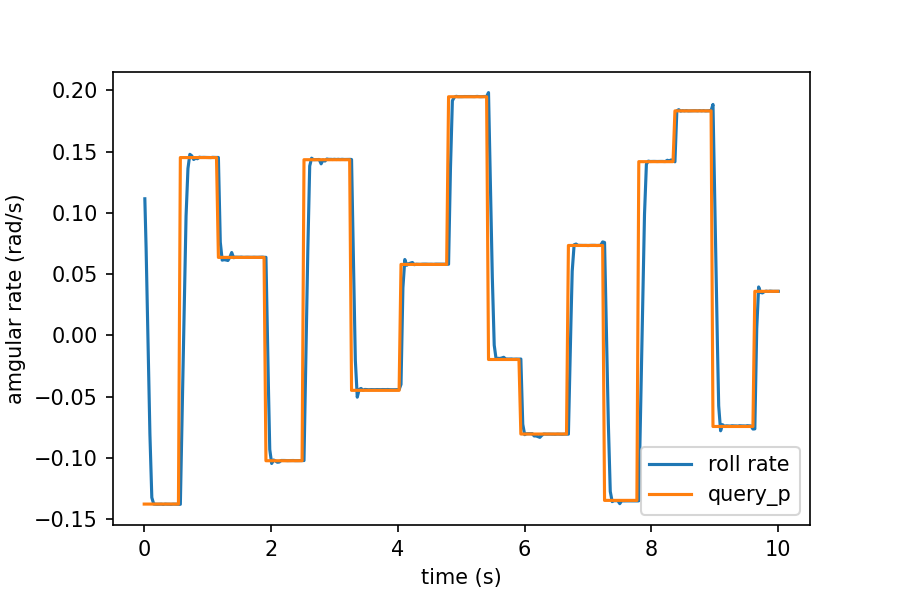
\includegraphics[width=\linewidth]{sac_16_16_cp_30}
\caption{Neural controller behaviour (sac, 2 layers, 16 neurons per layer, 3M iterations)}
\label{fig:samplespike}
\end{figure}
%\todo{Do we observe better performance on these "spikes" using SAC wrt DDPG, thanks to entropy regularization? NO EG}
%\todo{Can we have a similar picture for the same query but for the 2 PIDs? ARthur, first with other queries it is OK}



%\todo{Discuss the number of neural nets that comply with such complex specifications as low overshoot and offset for low rising time? Where there is no PID available? Arthur just a sentence on which 2 neural nets are "better" and for which thresholds.%Maybe a table of this number as a function of some of these constraints?
%}
When we filter the neural nets meeting or exceeding the performances of PID2, many networks remain, among which  %(best of the two neural nets), 
the best are:
\begin{itemize}
\item DDPG $64\times 64\times 64\times 64$ trained for 1500000  iterations (and also DDPG $32\times 32$, 400000 iterations\todo{Check}) on the three-dimensional observation space $(p-p_{sp}, q-q_{sp},r-r_{sp})$
%
%DDPG $32\times 32$ trained for 400,000 iterations 
    \item SAC $32\times 32 \times 32 \times 32$ (and SAC $32 \times 32$ and $16\times 16$ trained for 3000000 iterations coming very close) trained for  2900000 iterations on the same three-dimensional observation space
%    \item SAC $16\times 16$ ($32\times 32$ coming extremely close) trained for 3,000,000 iterations 
\end{itemize}
%These two networks perform much better on offsets and rising times, and very slightly worse on overshoots than our PIDs. These were obtained by filtering performance measures {\em OK rising t.} above 0.65, {\em OK off.} above 0.65 and {\em OK overshoot} above 0.85 
%(while PID2 is within the $\alpha$ percent of the query when reaching it, 90\% of the time, instead of 85\% for these best neural nets). %performs 0.9 on "OK overshoot".



\subsubsection{Training algorithm influence}

We observe in \Cref{fig:pidnnnominal}
%\todo{Add to Table 3 TD3 and PPO - Arthur later when we have PPO} 
that PPO and TD3 do not show as good performance as SAC (and even DDPG), moderating the conclusion of \cite{rl}, and the common belief that TD3 should improve performance of neural net control.
We have for now no explanation for this, largely because we have not been able (which is also the case in  \cite{rl}) to get rid of the overshoot spikes, even using SAC which does some amount of regularization, or TD3 which should lead to more stable solutions at, potentially, the expense of a slower convergence rate. In terms of optimal control, if the neural net controller were trained with correctness objectives\footnote{Future work to cope with this phenomenon includes improving the reward function using our STL observers, and adding some more regularization during training.}, these spikes would certainly be much smaller and appear only at the very beginning of plateaus. %\todo{Any explanation on this? Reduce optimism, reduces variance (so better knowledge of the states), more stable (more likely to converge) but takes more time to choose target policy.}. 

\subsubsection{Convergence of the training algorithms}

%\todo{Had to comment this because of missing figure - }
 We show in \Cref{table:perfsaciterations} the evolution of the three main performance measures, the OK overshoot, OK offset and OK rising time, for one of the best network architecture and training algorithm, SAC $32 \times 32$ neurons. 
 The three metrics improve quickly and almost stabilize in the first 1000000 iterations. 
 %\todo{Maybe this is because we take rising time in "an absolute manner", not wrt the last plateau? Remi, Arthur? A: rising time relative to stepsize is not expressible in STL as it is now, due to the fact that the threshold condition is embedded inside the aggregate subformula scope, and that the stepSize is only defined properly in the outer scope of the aggregate. This requires some extension of the language.}
 
%\todo{Graph with 3 curves, one for each observation space, and each curve being the avg overshoot, avg offset, avg rising time, just for SAC 32x32 if this is "the best"?}. 

%\todo{Put back the figure when we will have it}
%\begin{figure*}
%\missingfigure{Training iterations influence}
%\caption{Training iterations influence}
%\label{fig:perf-iteration}
%\end{figure*}
%\todo{To be done}

\todo{We observe also that the 
training speed seems to be better when neural nets are a bit deeper (but not too much?)}
%\todo{Show graph with a few lines corresponding to one perf measure (or reward?) one line per architecture from 1 layer 4 neuros to 4 layers 64 neurons per layer. Abscissa is the number of iterations}
\begin{figure}
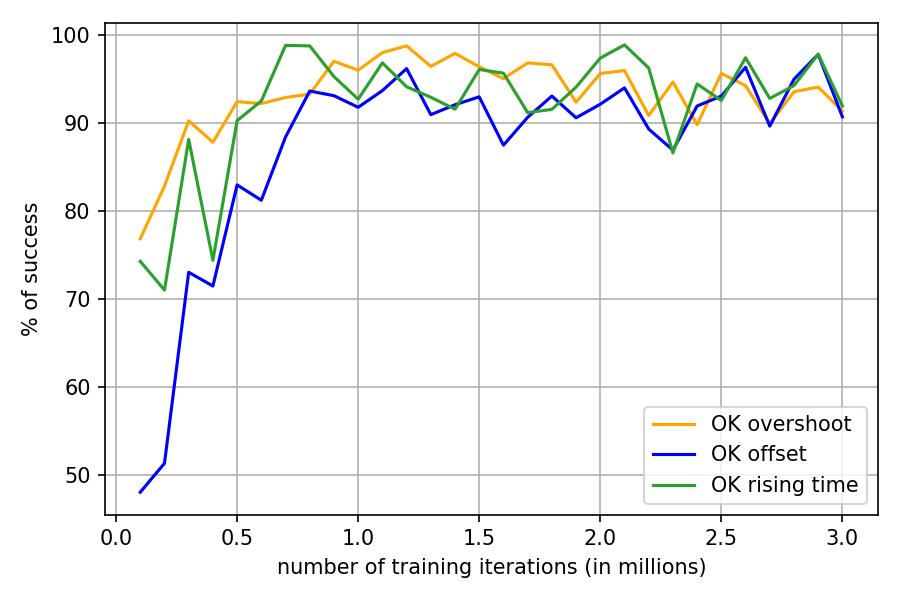
\includegraphics[width=\linewidth]{perf_sac_iterations_new.png}
\caption{Performance of SAC 32x32 on dim 3 observation space trained neural nets w.r.t. the number of iterations}
\label{table:perfsaciterations}
\end{figure}
\todo{Arthur: is this really the average relative offset performance ??? 40\% error seems enormous, overshoot should be at least greater than or equal to offset if the controller converges to the query }
\subsubsection{Observation state influence}

%As can be observed in this figure, and this is a general phenomenon of course,  
%more iterations are needed when the dimension of the observation space is higher\todo{Arthur, notes papier a partir de hiplot, a completer}.

Of course, the smaller dimension the observation state is, the better the quality of the sampling is, for the same number of iterations. %\todo{Arthur: table}
Still, we observe that using a Markovian state or the simpler three-dimensional state space $(err_p,err_q,err_r)$ does not change significantly the performance of the best neural nets obtained, see \Cref{fig:influencedim}, although the 3 dimension observation space gives slightly better performance overall. In fact, we even get a worse performance with the dimension 7 full state, mostly because of the difficulty to sample this higher dimensional space, and identify the subtle second-order effects of some of these states on angular rates.  %\todo{Table to put in Arthur}
\begin{csvtable*}{influence_nof_states3_new.csv}
\caption{Influence of the observable space dimension (all in \% except rising t. in seconds)}
\label{fig:influencedim}
\end{csvtable*}
% Could add the following figure sac_16_influence_dim.png
% that shows for sac 16x16, how the number of states influence the performances wrt the number of iterations
% This figure takes all the sac and ddpg with more at least 2 layers and 8 neurons per layer, and it averages it: sac_ddpg_influence_dim.png
%- DDPG best, SAC second best
\subsubsection{Neural net architecture influence}

First, we observe that almost none of the single-layer neural nets seem to converge to a correct controller (see e.g. \Cref{fig:architectures-iterations}). At 64 neurons, 1 hidden layer networks seem to exhibit some good behaviour, but still far from any of the e.g. two-layers neural nets. 
%\todo{it should be 32 instead of 8 no ? For now I have to leave the figure unfortunately - page limit constraints}
%Example of the behaviour of a single-layer neural net with 8 neurons is shown in \Cref{fig:sample1layer}\todo{Put in same format than the other figure which is \Cref{fig:samplespike}}, compare with \Cref{fig:samplespike} for a 32x32 neural net. %\todo{if these figures are to be compared, place them next to one another!!}

Still, 3-layers and even 4-layers networks do not seem to exhibit much better behaviour than the "best" 2-layers networks, with 16 or 32 neurons each, although they converge in a faster manner. %\todo{Check? We show evidence of this with a table or graph? just for SAC 3 states? Arthur figure simplifiee du slack du matin 4, 64, 16x16, 64x64, 4x4x4, 16x16x16, 64x64x64}. 
\begin{figure}
\centering
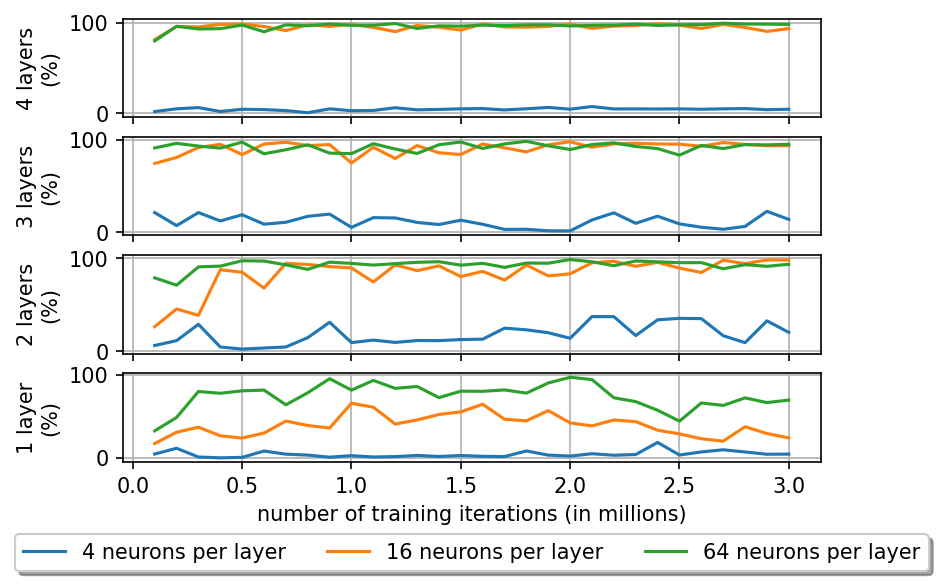
\includegraphics[width=\linewidth]{OK_rising_time_sac_architecture_iterations_new.png}
\caption{OK rising t. for our best SAC network wrt number of training iterations for different architectures}
\label{fig:architectures-iterations}
% Here SAC 32x32 3M iterations 3 states
\end{figure}
%\todo{(FXS) note: I managed to get all text on the same page by removing the text above the figures (duplicated in the captions)}
%We need to explore a very large hyper-parameters space and one very important dimension of this space is the depth of the MLPs used to implement the actor and the critic.
Recently Sinha et al. in~\cite{sinha2020d2rl} empirically observed the performance of SAC have a peak using 2 layers MLP and their explanation for this result relies on the Data Processing Inequality hence the fact that mutual information between layers decreases with depth. This will have to be further investigated in our framework. 
%It is interesting to observe according to the Information Bottleneck theory application to deep learning explained in \cite{Tishby2015DeepLA} the mutual information reduction between layers is actually an important feature to build a more synthetic latent representation which should help preventing overfitting. 
%Still \cite{sinha2020d2rl} focuses on DNN in supervised learning and we think this could be an important difference with respect to the reinforcement learning case. 


%This actually is consistent with what has also been recently observed in \cite{sinha2020d2rl} in the case of robotic control. 
 

%\begin{figure}
%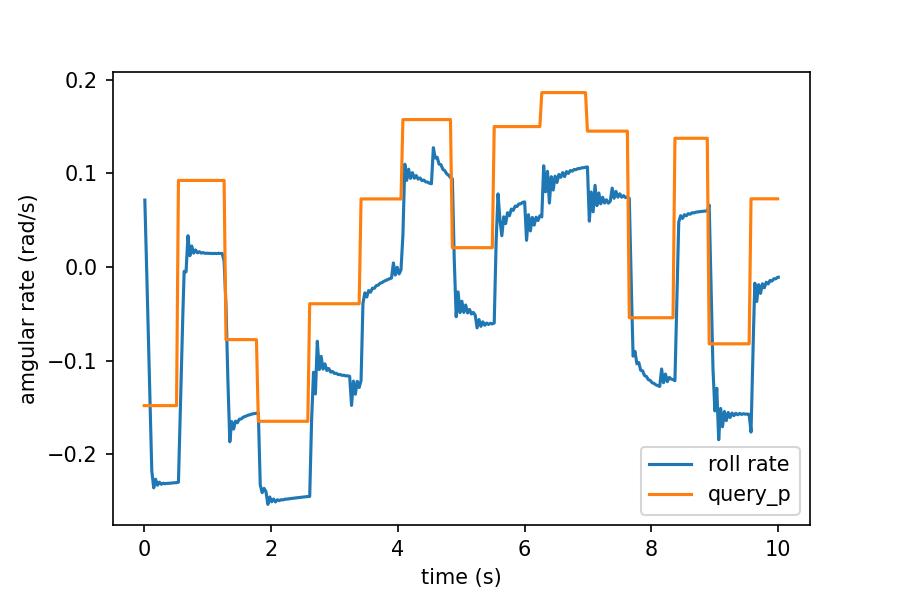
\includegraphics[width=\linewidth]{sac_8_cp_20.png} 
%\caption{Sample neural net (sac with 1 layer of 8 neurons) command trajectories and their  corresponding target angular rates trajectories.}
% Here SAC 32x32 3M iterations 3 states
%\label{fig:sample1layer}
%\end{figure}

%- 4 layers not better (even worse than 2)


%STL observers:

%Hard constraints 
%Baseline 2 PIDs : 

%- offset-rel-max : (mean of max on 100 episodes) explain : 

%- overshoot-rel-max

%- risingtime-all-max

%For the two PIDs: give values

%What do obtain for each criterion? :

%- offset only SAC with 1 hidden layer of 64 neurons, 2 layers with 32, 3 and 4 layers with 16... (check when we have 100 episodes)
%But when we want low rising time only few network work

%- overshoot max seems not very much correlated to the architecture of the neural net - but overshoot count is low for similar architectures as above (1 of 64, or 2 with 32 etc.)???? Always only for SAC and DDPG
%In fact, it seems that offset and overshoot are correlated

%- Show (quickly) that PPO does not work as well as DDPG/SAC? (similarly for TD3?)

%\paragraph{Remark} It is possible that given the discount factor of 0.99, tasks (here, episodic) of 1s take care of the reward in a nice way. Steps are every 0.03 seconds so at time 0, after 1s, the last reward has a discount of about 0.7 which is not negligible. After 20s, it is about 0.01s, which is negligible (so we see in the first iterations on 20s that at the end it does not follow at all the queries). To be checked (a way to do this is to ask for a discount factor of 0.9999999999 in continuous mode and see if this gets better)

%\todo{Is training with just one non null query for p, then for q, then for r more effective than training with combined targets?}

%\todo{Discuss easy vs medium query after training, also wrt to PIDs}

%\todo{Nicola, Arthur, R\'emi?}



\subsection{Performance of nominal-trained networks in non-nominal test cases}

\label{sec:expnonnominal}

\subsubsection{Robustness to motor failures}

We now assess the robustness of our PIDs and "best" neural nets (trained in nominal situations as discussed in  \Cref{sec:expnominal}) to partial motor failures, without training the neural nets nor changing the gains of PIDs to cope specifically for this situation. 

We report in \Cref{table:robustmotorfail} 
the same performance measures as the one used in the nominal case, in the test cases where motor 1 can experience a partial power loss, down to 80\% of its maximal power, at the start of any new plateau along the 20 second episodes that we are observing (which can contain about 30 different target angular states, or plateaus, to reach within a short time). We take maxima and averages of these measures on 100 such queries as before. %\todo{Check}

In case of partial motor failure, our best SAC trained neural net behaves much better than our two PIDs: it keeps on reaching plateaus within 0.5 seconds for about 94\% of the time, whereas even the best PID goes down to less than 60\% success rate. Our network is even better when it comes to satisfying offset constraints (82\% of the time) whereas the PIDs almost never comply. Performances concerning overshoot are comparable, even though the PIDs are very slightly better, but this only concerns cases where PIDs actually reach the target state, which is the case much less often. Basically, the best neural nets that have been trained under nominal conditions show very little degradation of performance when a partial failure occurs.  

%\begin{csvtable*}{pid_nn_nominal.csv}
%\caption{Robustness of best network and PID performance in case of partial motor failure}

%\end{csvtable*}
%\todo{Table to be changed - Same as table 3 but with non nominal cases}

%- Motor failure: looking again at offset-bad-count for now sac, 2 layers from 16 to 64 neurons each. PID is pretty bad (big count)
%(quantify for PID wrt neural net : PID at least 14 bad, for SAC it can be 0)

%Show some figures of response to queries for PID and for "best net". 

\subsubsection{Robustness to wind gusts}

We then assess the robustness of our PIDs and "best" neural nets (trained in nominal situations as discussed in  \Cref{sec:expnominal}) to wind gusts (described in \Cref{sec:aero}), without training the neural nets nor changing the gains of PIDs to cope specifically for this situation. 

We present in \Cref{table:robustwindgust}
%\todo{What is the last column? OK rising t.? Please change the csv accordingly and check? Why the 0 to 5 before the mode? Why has the table been shrunk, I thought it would be better to have the full table? I also changed the caption.}
the same performance measures than the ones used in the nominal case, when random wind gusts of magnitude up to 10 $m.s^{-1}$ can occur, from any fixed direction in the inertial frame, randomly chosen at the start of any new target plateau along the 20 second episodes that we are observing. We take maxima and averages of these measures on 100 such queries as before. %\todo{Check}

\begin{csvtable*}{non_nominal_test_new.csv}
\caption{Robustness of the best networks and PIDs in case of wind gusts and motor saturation (all in \% except rising t. in seconds)}
\label{table:robustnonnominal}
\label{table:robustwindgust}
\label{table:robustmotorfail}
\end{csvtable*}
%\todo{Table to be changed}

The PIDs and the neural nets exhibit the same kind of minor loss of performance, and the nominal trained neural nets are still far superior to the two PIDs. 
%PID1 performs again poorly, as before, with 7\% success for reaching plateaus and the performance. %Success for reaching plateaus is similar between our best SAC trained network and PID2, but PID2 never complies with the constraint we have on overshoot, that our network satisfies 62\% of the time while still enjoying a rising time which is only a third of the ones of the PIDs.
%Conclusion? wind gust: PID even worse ; 
%neural nets seem  much more adaptive to perturbations than PIDs. 

\subsection{Performance of non-nominal-trained networks}
%\todo{(FXS) Note: it is possible to gain space by shortening this heading}
%in nominal and non-nominal test cases
%}

\begin{csvtable*}{training_s_test_snew.csv}
\caption{Best networks trained for partial motor failures, tested under potential motor failures situations (all in \% except rising t. in seconds)}
\label{table:failnonnomnonnom}
\end{csvtable*}

\subsubsection{Training under partial motor failures}
In what follows, we train the attitude controller to sustain 
partial motor failures
%. For this, we suppose that we have on board a estimator of the state of each motor (that could also be learned).
%This could in fact be learned as well, using both the predicted command and states when there are no motor failures, and the (real) next state that is obtained, but this is outside the scope of this article. 
%This allows us to 
adding the magnitude of the power loss (1 extra dimension) to the observation states discussed in \Cref{sec:Markov}. We report the performance measures obtained in the non-nominal case in \Cref{table:failnonnomnonnom}. 
%\todo{To be changed}
The concern one may have is that, training the neural net in more various conditions (nominal and non-nominal), the resulting controller may exhibit lower performance. We thus report the same performance measures for neural nets trained with potential motor failures, in nominal situations, e.g. when no power loss happens, see  \Cref{table:failnonnomnom}

We see that we still achieve much better performance than PIDs, but that we are only similar and even slightly worse than the neural nets trained in nominal conditions, both in nominal conditions, compare \Cref{table:failnonnomnom} to  \Cref{fig:pidnnnominal}  and in non-nominal conditions, compare  \Cref{table:failnonnomnonnom} to \Cref{table:robustmotorfail}. Understanding this non intuitive behaviour and improving the training in this case is left for future work. 

\begin{csvtable*}{training_s_test_nnew.csv}
\caption{Performance of best networks trained with potential motor failures, and tested in nominal situations (all in \% except rising t. in seconds)}
\label{table:failnonnomnom}
\end{csvtable*}
%\todo{To be changed}

\subsubsection{Training under wind gusts}

In what follows, we train the attitude controller to sustain wind gusts up to 10 m.s$^{-1}$ in any direction, 
%We suppose, as in the case of motor failures, that we have an on board estimator that gives a value for the absolute wind that the quadcopter moves into. 
%There again, this can be done in numerous ways, by comparing a prediction of the next states with no wind, with the current observed states. 
%This allows us to 
adding to the observation states we discussed in \Cref{sec:Markov} the wind gust magnitude and directions (4 dimensions more) plus the linear velocities of the quadcopter ($u$, $v$ and $w$, 3 dimensions more) since they are necessary for determining the relative wind velocity. %, which is what ultimately counts as far as induced aerodynamic effects are concerned. 

We report the performance measures that we get in the non-nominal case in \Cref{table:windnonnomnonnom} and in the nominal case in \Cref{table:windnonnomnom}.
\begin{csvtable*}{training_w_test_wnew.csv}
\caption{Best networks trained for wind gusts conditions, tested under wind gusts conditions (all in \% except rising t. in seconds)}
\label{table:windnonnomnonnom}
\end{csvtable*}
%\todo{To be changed}
%As before, we report the same performance measures for neural nets trained with potential wind gusts, in nominal situations, e.g. when no wind gust happens, see  

We see that, the SAC and DDPG controller trained with potential wind gusts still behave about as well as the nominal controller, compare \Cref{table:windnonnomnom} to \Cref{fig:pidnnnominal}. Surprisingly, the best (SAC) network behaves slightly worse than the nominal-trained SAC network under wind gusts, compare \Cref{table:windnonnomnonnom} to \Cref{table:robustwindgust}, where we can see a slight drop of performance in e.g. {\em OK off.} and {\em OK overshoot}: it does not seem to be able to learn correctly how to stay close enough to the target plateau, in some cases. %\todo{Put some figures here from the corresponding tables}

\begin{csvtable*}[h!]{training_w_test_nnew.csv}
\caption{Best networks trained for wind gusts conditions, tested in nominal conditions (all in \% except rising t. in seconds)}
\label{table:windnonnomnom}
\end{csvtable*}
%\todo{To be changed}
%\todo{Wind gusts :
%Prefer vertical (in the inertial frame) winds?
%}

%\todo{Arthur with Eric?}

%\item Wind gust : (wind detection) direction, magnitude (continuous) on top of the state representation we choose in the nominal case
%\end{itemize}

%\todo{Discuss some "success" measures (hidden STL formulas). Discuss reachability (in some simple conditions - linked with the query generator, given a minimum dwell time), Sherlock/RINO.}

\section{Conclusion}

We have presented a complete study of learned attitude controls for a quadcopter using reinforcement learning. In particular we extend previous results by modeling partial motor failure as well as wind gusts, and generating extensive tests of various network architectures, training algorithms and hyperparameters using a flexible and robust experimental platform. We also present a precise evaluation mechanism based on robust signal temporal logic observers, which allows us to characterize the best options for training attitude controllers.
Results show that learned controllers exhibit high quality over a range of query signals, and are more robust to perturbations than PID controllers.
%Future work includes for example further study of the training scenarios (including more non-nominal cases) \todo{Future work needs to be written}.

The immediate next step will be to start
using STL-derived reward signals during training on the most promising
architectures, and try to improve training under non-nominal situations. 

Finally, because we use an explicit ODE model, we can hope to discuss formal reachability properties of the complete controlled system, using or elaborating on approaches such as \cite{sherlock} and \cite{goubault_putot}. 

%Improve reward using temporal logics specification as in \cite{TLRL1} and \cite{Belta}. 
%(this is just the beginning - it will be most probably much better to use temporal logic specification with possibly inner/outer approximations, for computing e.g. the reward function, during training)

%(just the beginning also for verification with a neural net in the control loop)


%\clearpage
\todo{(FXS) I am not enough of an expert in \LaTeX, but when we use the clearpage command all tables are on the same page, however bibliography is split in a weird way; EG: yes, I did put a clear page because this was weird, but it is also weird with a clear page. Also bib and appendix do not count within the 10 pages limit, so I thought a clear page would do. Let me try something else.}
%\newpage
%\newpage
\pagebreak
\bibliography{main}

\appendix

\section{Parameters}
\label{sec:parameters}

The physical and constant parameters for the crazyflie are obtained by merging data from \cite{quadcopter_model} and \cite{nanoquadcop}.

\begin{table}[h]
\centering
\begin{tabular}{@{}llrr@{}}
    \toprule
    Param & Description & Value & Unit \\
    \midrule
    $I_x$ & Inertia about x-axis & \num{1.657171e-5}  & \si{\kilo\gram\square\metre} \\
    $I_y$ & Inertia about y-axis & \num{1.6655602e-5} & \si{\kilo\gram\square\metre} \\
    $I_z$ & Inertia about z-axis & \num{2.9261652e-5} & \si{\kilo\gram\square\metre} \\
    $m$ & Mass & \num{0.028} & \si{\kilo\gram} \\
    $g$ & Gravity & \num{9.81} & \si{\metre\per\square\second} \\
    $C_T$ & Thrust Coefficient & \num{1.285e-8}  & \si{\newton\per\square\radian\square\second} \\
    $C_D$ & Torque Coefficient & \num{7.645e-11} & \si{\newton\per\square\radian\square\second} \\
    $C_1$ & PWM to $\Omega$ factor & \num{0.04076521} & - \\
    $C_2$ & PWM to $\Omega$ bias   & \num{380.8359}   & - \\
    $h$ & z rotor wrt CoG & 0.005 & \si{\meter} \\
    $d$ & Arm length & $0.046/\sqrt{2}$ & \si{\meter} \\
    $p_{max}$ & Maximum motor PWM & \num{65535} & - \\
    \bottomrule
\end{tabular}
\caption{Parameters for the model}
\label{params2}
\end{table}

%The PWM signals being encoded as 16-bit numbers between $0$ and $65535$, the following orders of magnitude result from the above equations:
%\begin{gather*}
%0 \leq \omega_i \leq \SI{3.1e3}{\radian\per\second} = \SI{2.9e4}{ rpm} \\
%0 \leq F_i \leq \SI{0.12}{\newton} \implies F = \sum F_i \leq 0.48\ N \text{ and }\tfrac{F}{m} \leq \SI{18}{\meter\per\square\second} \\[1em]
%\begin{multlined}
%(thrust,\ cmd_{\phi},\ cmd_{\theta},\ cmd_{\psi}) \in [0,\ p_{max}]  \times [-p_{max},\ p_{max}] \\ \null\hfill \times [-p_{max},\ p_{max}]\times \left[-\frac{p_{max}}{2},\frac{p_{max}}{2}\right]
%\end{multlined}
%\end{gather*}


The drag coefficients are \cite{nanoquadcop}:
\begin{equation*}
K =
\begin{pmatrix}
-9.1785 & 0 & 0 \\
0 & -9.1785 & 0 \\
0 & 0 & -10.311
\end{pmatrix}
10^{-7} kg.rad^{-1}
\end{equation*}
%\paragraph{Note} Smaller coefficients for lateral drag than in \cite{nanoquadcop} since simulations showed these were probably over-estimated in this simple drag model. 

The maximal magnitudes of states are given in \Cref{params1}:
%\todo{EG : I am in the process of changing this a little! E.g. much larger bounds for $z$ (we do not care if the quadcopter falls, in this study)}
%\todo{To be discussed : singularity at angle of $\frac{\pi}{2}$ ; but big angular velocities are alright - we could still shrink down the bounds of angular velocities, but then the inertial effect will be less visible... let's see...Look also at table 3.3. of \cite{simtoreal}}
%\todo{Remark : the attitude controller inside the crazyflie works at 500 Hz, so delta command could be changed to 0.002s?}

%Global hypothesis : PID is constrained to saturate at 80\% of the maximal thrust (to give some slack to attitude controls)

%Command frequency : 33 Hz
%Integration time : 0.01s 

%Wind gusts : $A_g\leq 1 m.s^{-1}$, $0.1s \leq\delta\leq 0.2s$ \todo{Checked with respect to the code}

%Hypothesis : small angles and small angular rates

\begin{table}[H]
    \centering
    \begin{tabular}{@{}llrr@{}}
        \toprule
        Variable & Unit & Lower Bound & Higher Bound \\
        \midrule
        $z$ & \si{m} & -1000 & +inf\\
        $u$ & \si{m.s^{-1}} & {-30}  & {30}\\
        $v$ & \si{m.s^{-1}} &  {-30 }& {30}\\
        $w$ & \si{m.s^{-1}} & {-30}  & {30}\\ 
        $\phi$   & \si{\radian} & ${-\pi}$ & ${\pi}$\\
        $\theta$ & \si{\radian} & ${-\pi}$ & ${\pi}$\\
        $\psi$   & \si{\radian} & ${-\pi}$ & ${\pi}$\\
        $p$ & \si{\radian.s^{-1}} & ${-5\pi}$ & ${5\pi}$\\
        $q$ & \si{\radian.s^{-1}} & ${-5\pi}$ & ${5\pi}$\\
        $r$ & \si{\radian.s^{-1}} & ${-5\pi}$ & ${5\pi}$\\
        $cmd_\phi$   & PWM & -400 & 400\\
        $cmd_\theta$ & PWM & -400 & 400\\
        $cmd_\psi$   & PWM & -1000 & 1000\\
        $F$ & \si{\newton} & 0 & 52428\\
        \bottomrule
    \end{tabular}
    \caption{State and action space bounds}
    \label{params1}
\end{table}

The base PID1 we have been comparing our controller to is given in \cite{goubault_putot}:
\begin{equation}
\label{eq:control1}
\left\{
\begin{aligned}
thrust &= 1000 \big(25(2(z_{sp} - z) - w) \\ & \qquad + 15 \smallint (2(z_{sp} - z) - w)\dt\big) + 36000 \\
cmd_{\phi} &= 250 (p_{sp} - p) +  500 \smallint (p_{sp} - p) \dt \\
cmd_{\theta} &= 250 (q_{sp} - q) +  500 \smallint (q_{sp} - q) \dt \\
cmd_{\psi} &= 120 (r_{sp} - r) + 16.7 \smallint (r_{sp} - r) \dt
\end{aligned}
\right.
\end{equation}
%Hypothesis : big angles and angular rates



\end{document}











\newpage

\section{Properties of the learned controller}
\todo{Most probably next paper}


\todo{Arthur with Eric?}

\subsection{Reachability properties}

\label{sec:reachability}

\todo{Sylvie?}

\todo{What we are doing for now can be considered as some sort of robustness properties of the neural nets within the control loop. Also, a good idea would actually to use also the range analysis of networks to see if indeed, for a subset of (not too big) values of $p$, $q$ and $r$, and when having reached the target attitude, we get very very small commands (some sort of specification to be checked).}

Robustness test for neural net controllers (around queries).

Start state with $z \in [-0.05,0.05]$, $p, q, r \in [-0.01,0.01]$. Target states are $z=0.1$, $p=-0.1$, $q=0.1$, $r=0.1$.

\Cref{PID2,PID2-2} give the corresponding (inner and outer) flowpipes on 3 seconds for the second PID. 

\Cref{PID1,PID1-2} give the corresponding (inner and outer) flowpipes on 3 seconds for the second PID. 

The first PID is very agressive with very good performances in roll, pitch and yaw, and a huge overshoot in $z$. The PID of \cite{goubault_putot} is much less agressive, but has a much more stable altitude control. 

\begin{figure}[h]
    \centering\noindent
    \begin{subfigure}[t]{\linewidth}
        \centering
        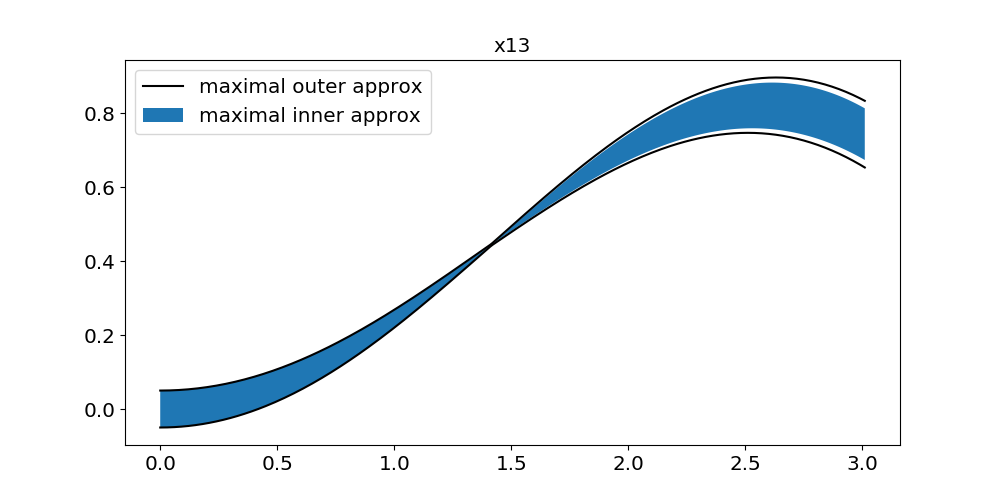
\includegraphics[width=0.49\linewidth]{x13_min_max_PID2}\hfill
        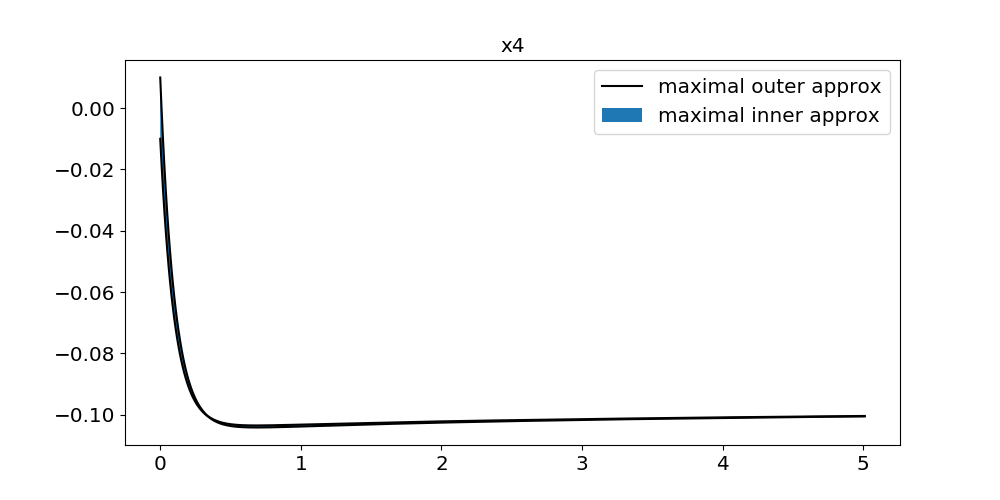
\includegraphics[width=0.49\linewidth]{x4_min_max_PID2}
        \caption{$z$ and $p$}
        \label{PID2-zp}
    \end{subfigure}
    \hfill
    \begin{subfigure}[t]{\linewidth}
        \centering
        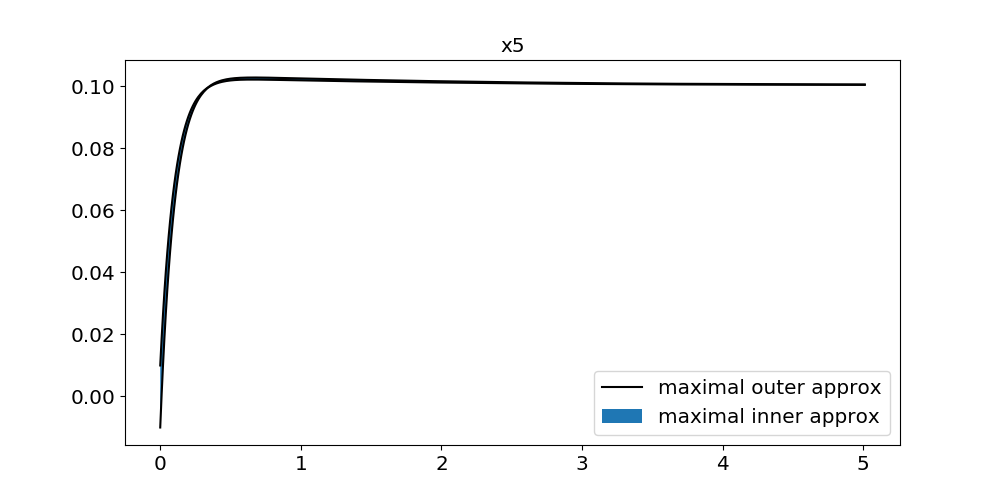
\includegraphics[width=0.49\linewidth]{x5_min_max_PID2}\hfill
        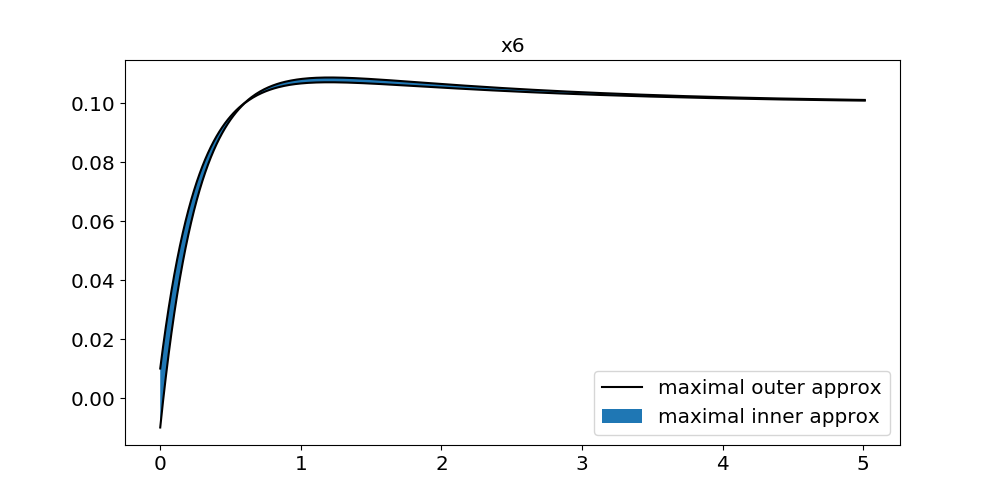
\includegraphics[width=0.49\linewidth]{x6_min_max_PID2}
        \caption{$q$ and $r$}
        \label{PID2-qr}
    \end{subfigure}
    \caption{PID2}
    \label{PID2}
\end{figure}

\begin{figure}[h]
    \centering\noindent
    \begin{subfigure}[t]{\linewidth}
        \centering
        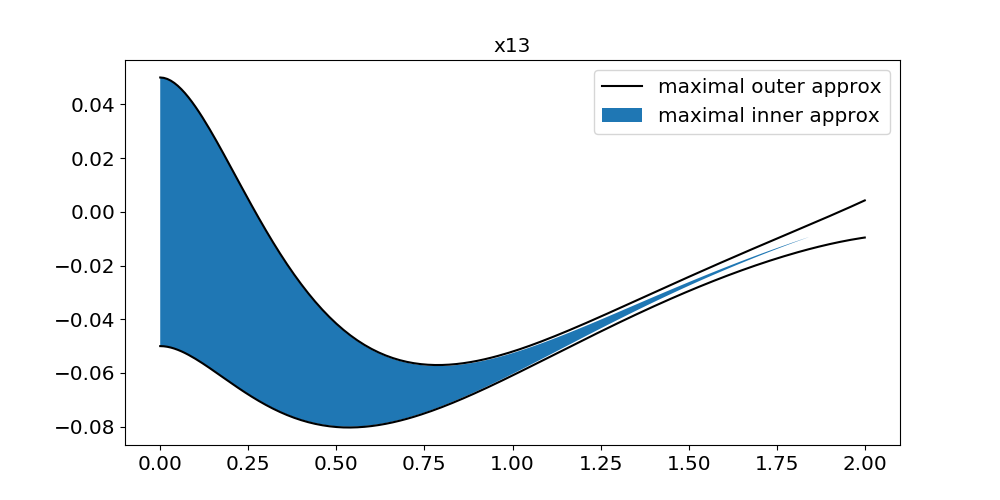
\includegraphics[width=0.49\linewidth]{x13_min_max_PID1}\hfill
        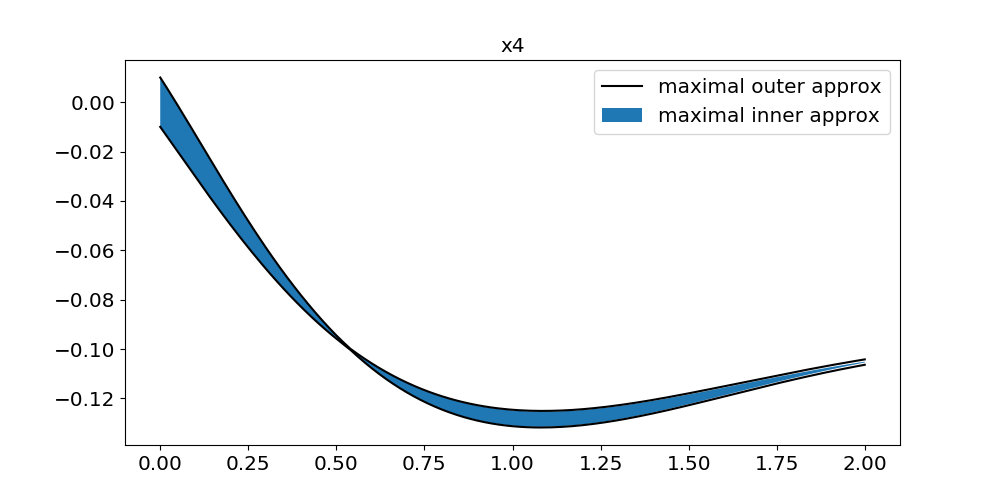
\includegraphics[width=0.49\linewidth]{x4_min_max_PID1}
        \caption{$z$ and $p$}
        \label{PID1-zp}
    \end{subfigure}
    \hfill
    \begin{subfigure}[t]{\linewidth}
        \centering
        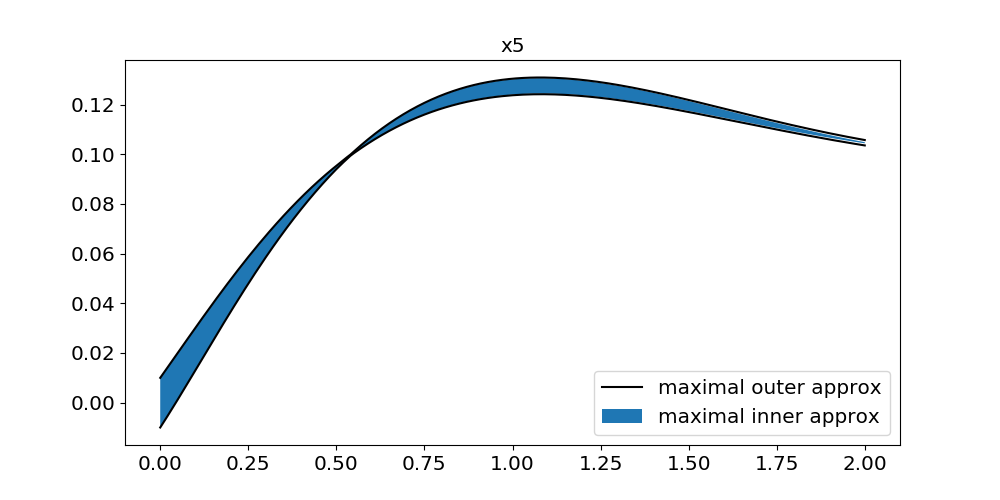
\includegraphics[width=0.49\linewidth]{x5_min_max_PID1}\hfill
        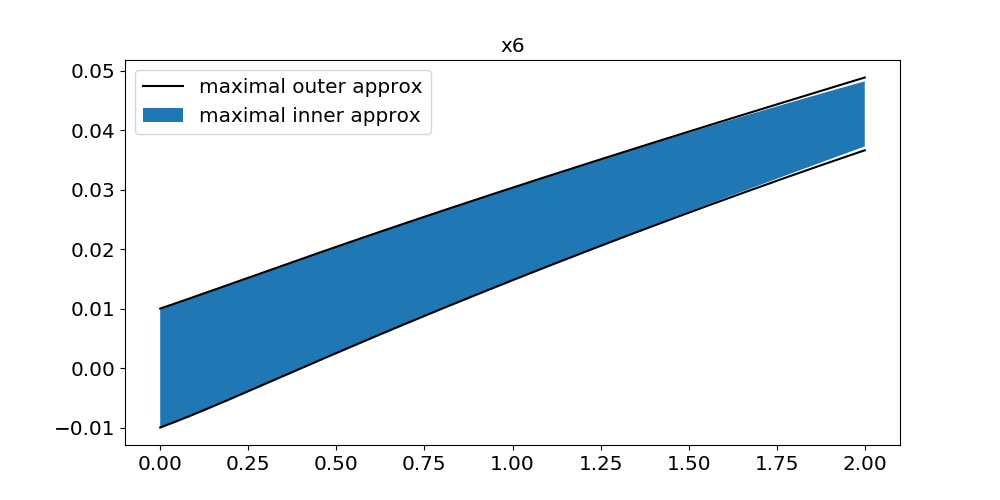
\includegraphics[width=0.49\linewidth]{x6_min_max_PID1}
        \caption{$q$ and $r$}
        \label{PID1-qr}
    \end{subfigure}
    \caption{PID1}
    \label{PID1}
\end{figure}

We show in \Cref{PID2-wind,PID2-wind-2} the effect of a constant diagonal (in the inertial frame) side wind of about \SI{6}{km.h^{-1}}. Yaw is still controllable, but pitch and roll exhibit a large overshoot. 

\begin{figure}[h]
    \centering\noindent
    \begin{subfigure}[t]{\linewidth}
        \centering
        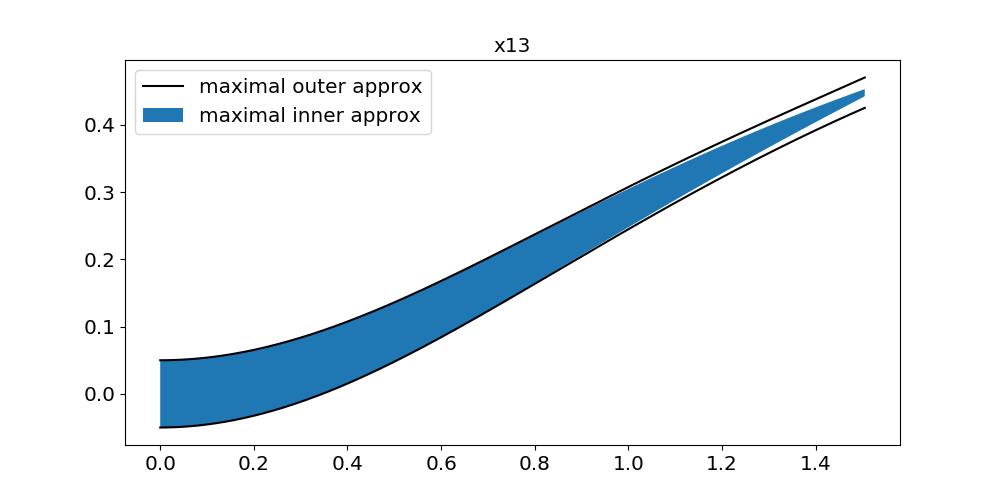
\includegraphics[width=0.49\linewidth]{x13_min_max_PID2_wind_1-1-1}\hfill
        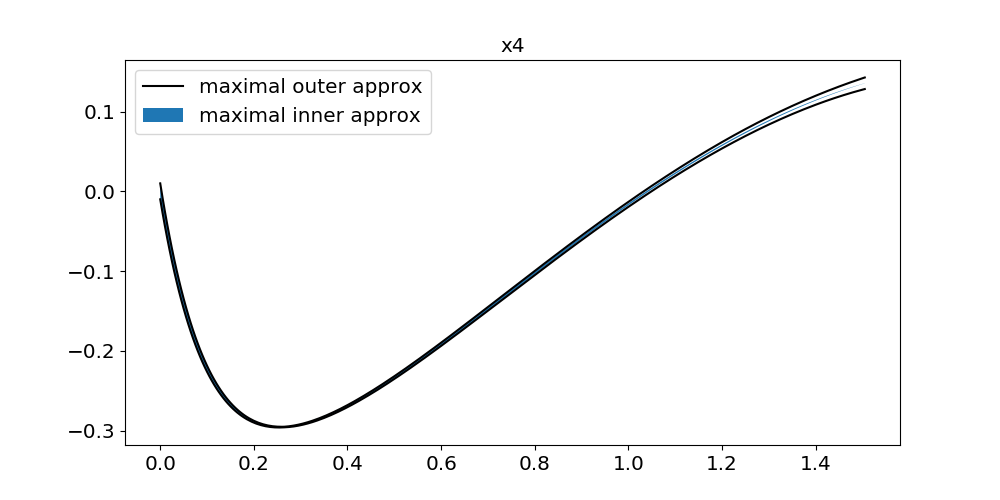
\includegraphics[width=0.49\linewidth]{x4_min_max_PID2_wind_1-1-1}
        \caption{$z$ and $p$}
        \label{PIDw-zp}
    \end{subfigure}
    \hfill
    \begin{subfigure}[t]{\linewidth}
        \centering
        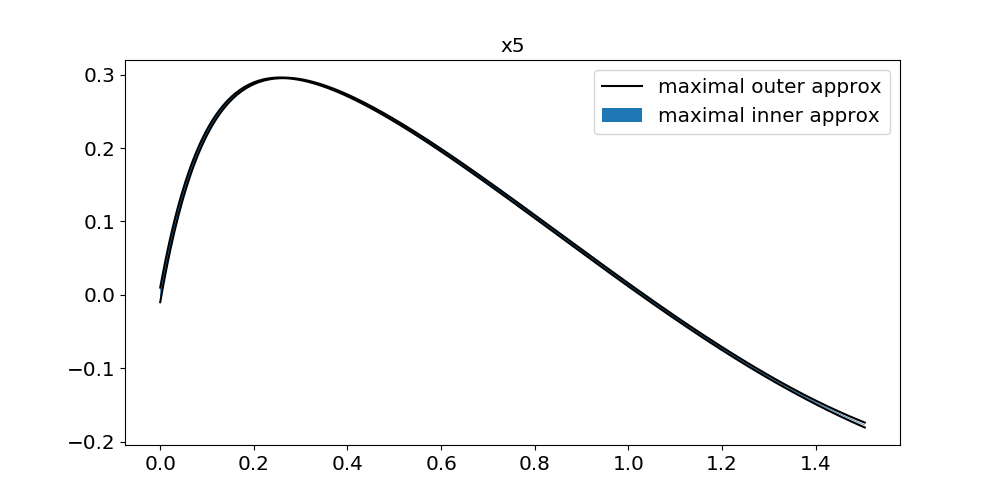
\includegraphics[width=0.49\linewidth]{x5_min_max_PID2_wind_1-1-1}\hfill
        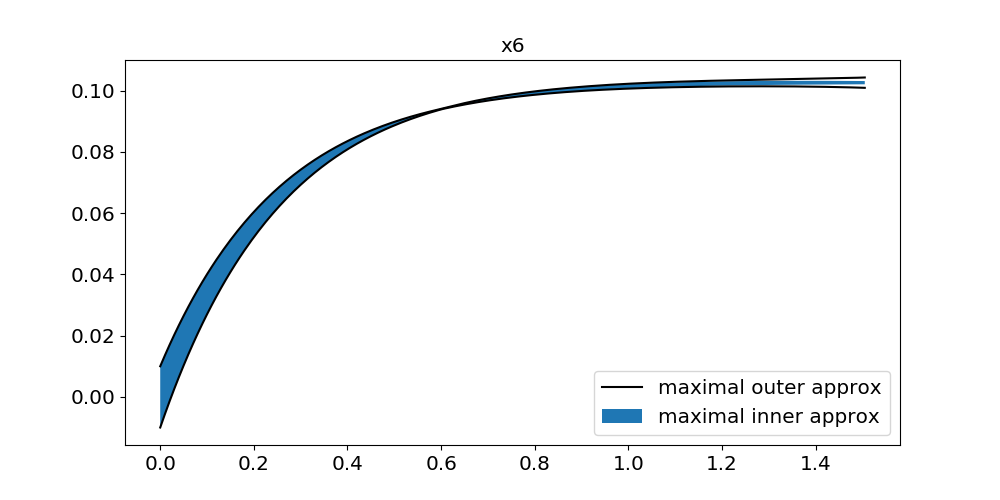
\includegraphics[width=0.49\linewidth]{x6_min_max_PID2_wind-1-1-1}
        \caption{$q$ and $r$}
        \label{PIDw-qr}
    \end{subfigure}
    \caption{PID wind}
    \label{PIDw}
\end{figure}

%\section{Learning in non-nominal cases}

%\begin{itemize}
%    \item Discuss degradation of performances for a nominal controller that is trained to also cope with partial motor failures or wind gusts (towards continual learning?)
%    \item Discuss success measures and simple reachability (Sherlock / RINO)
%\end{itemize}

\end{document}


\section{Material to be discussed}

\subsection{Old section on training and remarks}

\begin{figure}[htbp]
    \centering
    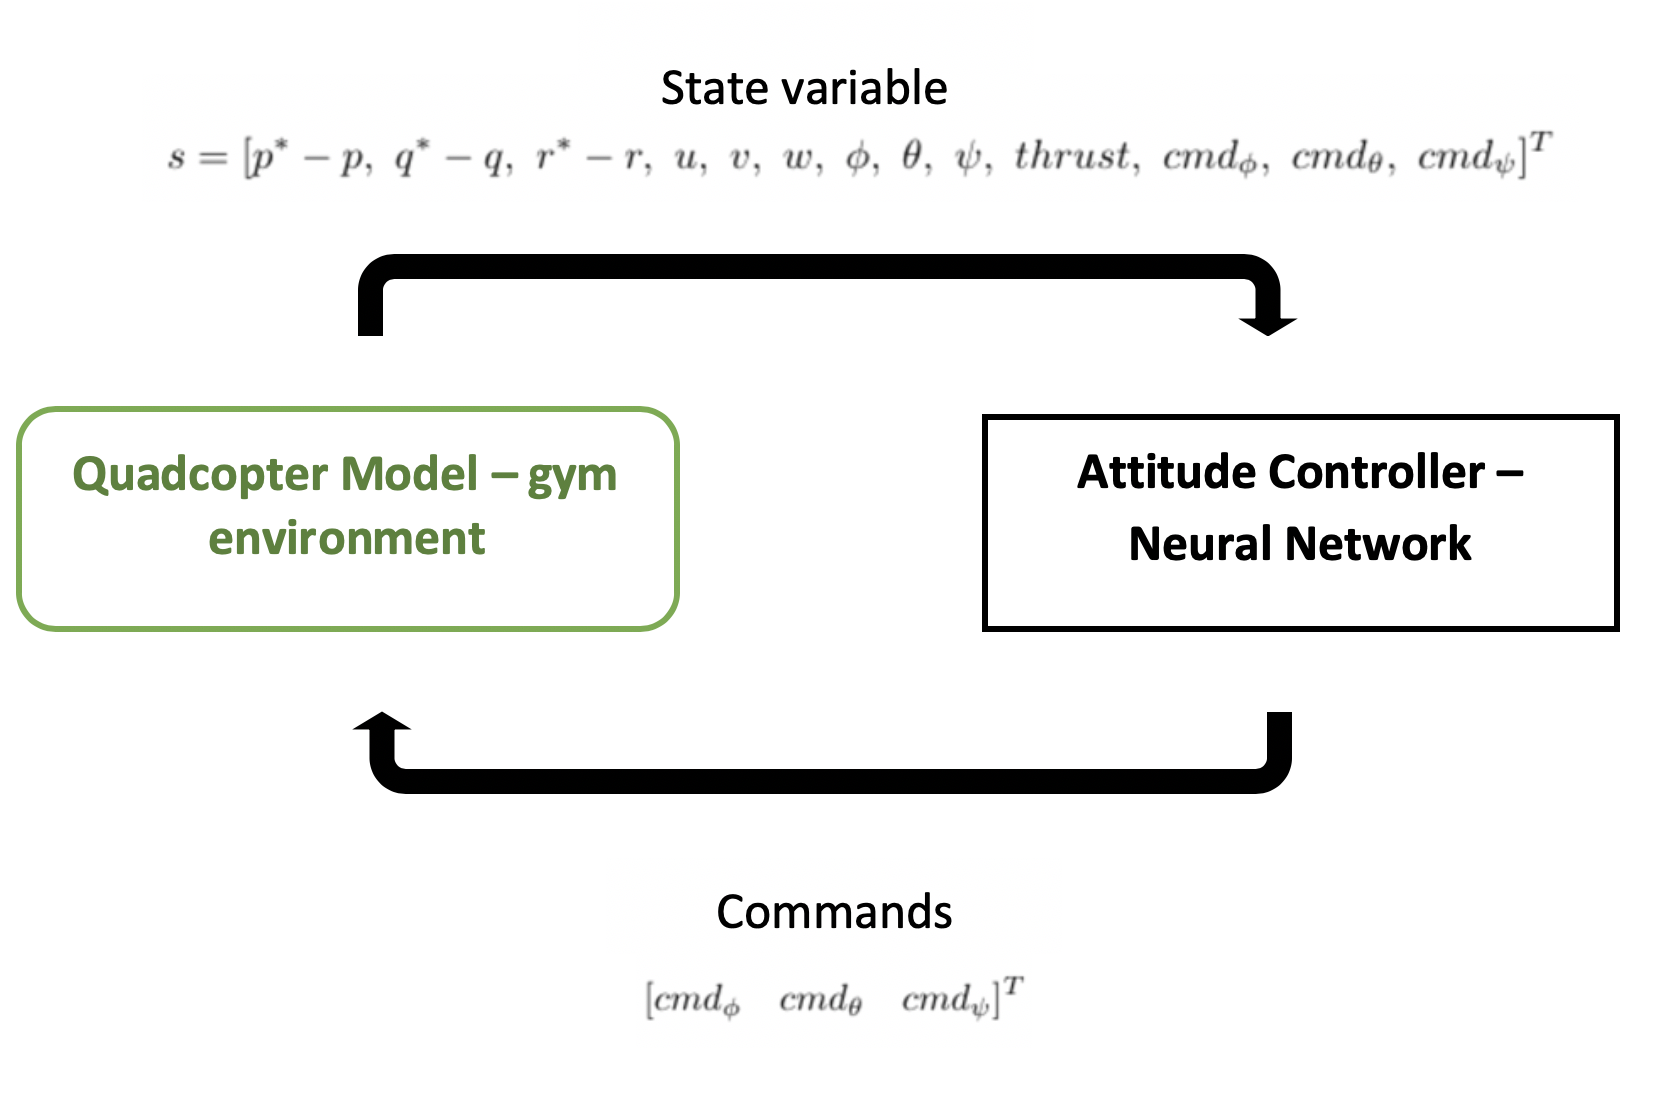
\includegraphics[width=\linewidth]{schema2}
    \caption{Attitude Control Loop for each time step, the attitude controller receives queries which he must make the quadcopter model attain.}
    \label{fig:loop}
\end{figure}

The RL agents/controllers described further take as input a variable describing the current quadcopter state $s$ (13-dimensional vector, cf. \Cref{state}) and return an action to be taken by the aircraft to get closer to its angular rate goal $\Omega^*$: 
$a =(cmd_\phi, cmd_\theta, cmd_\psi)= Agent(s)$. 
The state variable $s$ is then updated according to $a$ and the \Cref{eq:dynamic}. Then, another action can be computed and so forth. 

As state variable for the RL task, we used a size 13 concatenation of the angular rate error $\Omega^* - \Omega = (p^* -p,\ q^* - q,\ r^* - r)$ with the quadcopter's orientation, speed and the four control values: $s = (p^* -p, q^* - q, r^* - r,\ u, v, w, \phi, \theta, \psi, thrust, cmd_\phi,\ cmd_\theta,\ cmd_\psi)$. 
These variables are included in the state variable because they all affect attitude control. In \cite{rl}, only $\Omega^* - \Omega$ and the four control values are used, most likely to simplify the task and fasten convergence. 
\todo{Check this is env0. Some experiment to be made here. Some past states were used in \cite{rl}? To be checked}
Still, the choice of removing the current angular orientation $[\phi \quad \theta \quad \psi]^T$ is hard to explain, as the quadcopter's stability heavily depend on the angular orientation. 
\todo{Discuss state - past states should also be considered - should also experiment without the angular orientation to make sure }

We will train two kind of controllers: one is an aggressive controller, where target angular rates can be very important (see \Cref{sec:parameters}), and one where the controller will only be used for small target angular rates. In the second case, the second order effect, that couple all states of the quadcopter dynamics, will be negligible. 

\paragraph{Remark:}
First, using our neural net architecture, we do not have any "feature extraction", so it seems really important, looking at the first  experiments, to choose "the right states to observe", from the start. 

Expanding the coefficients for angular velocities in the equations of the dynamics, we have : 
$\dot{p}=-0.760697* q * r + (-8.38277868313e-3)*z*cmd_{phi}  - (4.19138934156e-3)*w*cmd_{phi} + (2.51483360494e-3)*zI*cmd_{phi} + 0.0159846477606*cmd_{phi} - (1.67655573663e-7)*cmd_{theta}*cmd_{psi}$
			 
$\dot{q}=0.761902* p * r + (-8.34055576802e-3)*z*cmd_{theta} - (4.17027788401e-3)*w*cmd_{theta} + (2.50216673041e-3)*zI*cmd_{theta} + 0.0159041352657*cmd_{theta} - (1.66811115361e-7)*cmd_{phi}*cmd_{psi}$
    
$\dot{r}=-0.002867* p * q + (-1.73667282186e-3)*z*cmd_{psi} - (8.68336410928e-4)*w*cmd_{psi} + (5.21001846557e-4)*zI*cmd_{psi} + (3.31156343047e-3)*cmd_{psi} - (8.68336410931e-9)*cmd_{theta}*cmd_{phi}$

The terms in $z$, $zI$ and $u$, $v$, $w$ comes from the expansion of the formula giving $thrust$. So in terms of immediate dependencies, we might find it a good idea to represent in the state, $p$, $q$, $r$, (as well as the targets of angular velocities, or even the differences of angular velocities with target velocities) $z$, $zI$, $u$, $v$, $w$, or just $p$, $q$, $r$, $thrust$? 
We might also want to "regularize" the commands using past commands $cmd_{phi}$, $cmd_{psi}$, $cmd_{\theta}$ (to be checked - probably a bad idea since the current experiments).

In theory, using MLP with RELU, we should be able to learn any piecewise affine function, so we can hope that during training, it will learn the best piecewise affine approximation of an "optimal" controller. 
When the angular velocities $p$, $q$ and $r$ are "small" enough, given the expanded formulas above, we should have the property that $cmd_{\phi}$, $cmd_{\psi}$ and $cmd_{\theta}$ are 0 when we have reached the target angular rates. Otherwise, if $p$, $q$, $r$ are sufficiently important, we still have to counter-effect the induced moment (of order two, terms in $pq$, $qr$ and $pr$). 

As seen in the equations above, the order 2 influence of $z$, and of the linear velocities, seem to be rather negligible, as expected, with respect to the most important term, which is the linear term in $cmd_{phi}$ (resp. $cmd_{theta}$, $cmd_{psi}$). Is is possible that the training does not manage well to represent the fact that when $p$, $q$ and $r$ are small, the 
influence of $z$ (same for $zI$, and the linear velocities) should be in a domain of the piecewise affine function where it is zero. 

Given the coefficients above (that is, the inertia matrix in particular), and given that 
the commands $cmd_{\phi}$, $cmd_{\psi}$ and $cmd_{\theta}$ between -65536 and 65536 (to be checked), it seems that when $p$, $q$ and $r$ are less than 1 $rad/s$, this effect is rather negligible. It is also possible that the training does not converge well enough to account for these second-order effects. 

So overall, it is possible that the training behaves better with a smaller observation state, the smallest one being 
$p-p_{sp}$, $q-q_{sp}$, $r-r_{sp}$. We should try also the full state, but also $p$, $q$, $r$, $p-p_{sp}$, $q-q_{sp}$, $r-r_{sp}$, $thrust$, typically, at least when $p_{sp}$, $q_{sp}$, $r_{sp}$ can be big enough (more than 1 $rad/s$?)? And other combinations... It would be nice to have "success measures" and not only figures, to assert the quality of these choices, before going to the reachability analysis. 

Two reward functions were considered:
\begin{gather*}
r_1(s) = - clip \Big( \frac{1}{3\Omega_{max}} \left\lVert \Omega^* - \Omega \right\rVert_1,\ 0,\ 1 \Big) \\
r_2(s) = r_{step} - clip \Big( \frac{1}{3\Omega_{max}} \left\lVert \Omega^* - \Omega \right\rVert_1,\ 0,\ 1 \Big)
\end{gather*}
with $clip(x, a, b) = max(min(a, x), b)$, and $\Omega_{max} = \pi$ \\
\todo{clip is necessary? tanh normalization? Other stuff?}
$r_1$ is the one used in most of our experiments. It is negative as it was designed for episodic tasks where the quadcopter cannot crash in less than $1.0$ second (extreme attitude commands would be required). 

We considered $r_2$ --- with $r_{step} \in [0.1, 1.0]$ --- for continuous training because it would make the quadcopter's flight last longer despite hard angular rate queries. Indeed, in this case, the use of a negative reward could result in an agent that makes the quadcopter crash as fast as possible, thus preventing its reward from decreasing later. However, with $r_2$, as expected, the quadcopter becomes a bit less responsive to angular rate queries. \\ 
\todo{Check this is still the case}

\onecolumn
\listoftodos{}

\end{document}
